\documentclass[a4paper]{article}

%%%%%%%%%%%%%%%%%%%%%%%%%%%%%%%%%%%%%%%%%%%%%%%%%%%%%%%%%%%%%%%%%%%%%%%%%%%%%
% Packages

\usepackage[margin=18mm]{geometry}
\usepackage{amsmath}
\usepackage{amssymb}
\usepackage{amsthm}
\usepackage{algpseudocodex}

\usepackage{booktabs}
\usepackage{tabularx}
\usepackage{array}
\usepackage{enumitem}

\usepackage{chemfig}
\usepackage{xcolor}
\usepackage{framed}

\usepackage{pdflscape}

\usepackage{pgfplots}
\usepackage{tikz}
\usetikzlibrary{arrows, matrix, backgrounds, calc, positioning, shapes}

% Match the IDSC vibe with the sans-serif font
\usepackage[T1]{fontenc}
\usepackage{cmbright}
\renewcommand*\familydefault{\sfdefault}

%%%%%%%%%%%%%%%%%%%%%%%%%%%%%%%%%%%%%%%%%%%%%%%%%%%%%%%%%%%%%%%%%%%%%%%%%%%%%
% Custom Macros

\newcommand{\todo}[1]{\texttt{TODO: #1}}

\newcommand{\T}{\mathsf{T}}
\newcommand{\E}[2][]{\mathbb{E}_{#1}\left\{#2\right\}}
\newcommand{\given}{\mid}
\newcommand{\ind}{~\bot~} % independent variables
\newcommand{\co}[1]{[\text{#1}]} % concentration

\DeclareMathOperator{\st}{such~that}
\DeclareMathOperator{\tr}{tr}
\DeclareMathOperator{\rank}{rank}
\DeclareMathOperator{\pa}{pa} % parent
\DeclareMathOperator{\de}{de} % descendant
\DeclareMathOperator{\sign}{sign}

\theoremstyle{plain}
\newtheorem{thm}{Theorem}[section]
\newtheorem{lemma}{Lemma}[section]
\newtheorem{prop}{Proposition}[section]

\theoremstyle{definition}
\newtheorem{defn}{Definition}[section]
\newtheorem{alg}{Algorithm}[section]

\theoremstyle{remark}
\newtheorem*{example}{Example}
\newtheorem*{remark}{Remark}

%%%%%%%%%%%%%%%%%%%%%%%%%%%%%%%%%%%%%%%%%%%%%%%%%%%%%%%%%%%%%%%%%%%%%%%%%%%%%
% Metadata

\title{Notes of Computational Systems Biology}
\author{Naoki Sean Pross}

\begin{document}

\maketitle

\begin{abstract}
  These (rather rough) notes are based on the contents of the course
  \emph{Computational Systems Biology} taught by Jörg Stelling at ETH Zürich
  and the book \emph{System Modelling in Cellular Biology} (ISBN
  \texttt{978-0-262-19548-5}). However, at the time of writing the author has
  practically zero biology knowledge. Therefore, these note are very likely to
  be skewed towards the mathematical content of the course, since that is the
  only part that he understands.
\end{abstract}

\tableofcontents

\clearpage

%%%%%%%%%%%%%%%%%%%%%%%%%%%%%%%%%%%%%%%%%%%%%%%%%%%%%%%%%%%%%%%%%%%%%%%%%%%%%

\section*{Notation}

\begin{center}
  \renewcommand{\arraystretch}{1.5}
  \begin{tabularx}{\linewidth}[t]{%
      >{\(\displaystyle}l<{\)} X >{\(\displaystyle}p{34mm}<{\)}
    }
    \toprule
    \textbf{Symbol}
      & \bfseries Meaning
      & \textbf{Other Commonly}\newline \textbf{Used Symbols}
      % & \bfseries Notes
      \\
    \midrule
    \multicolumn{2}{l}{\itshape Probability Theory} \\
    x \in \mathcal{X}, y \in \mathcal{Y}
      & Random variables $x$ and $y$, that can take values from $\mathcal{X}$
        and $\mathcal{Y}$ respectively.
      \\
    x \given y
      & Random variable $x$ conditioned on $y$ (``$x$ given $y$'').
      \\
    x ~\bot~ y
      & The random variables $x$ and $y$ are independent.
      \\
    p_x(\bar{x})
      & Probability density function of $x$ evaluated at $\bar{x}$. We may
        sometime simplify the notation and just write $p(x)$ if it clear from
        the context.
      & P(x), \Pr(x), \mathbb{P}(x)
      \\
    p_{x \given y}(\bar{x} \given \bar{y})
      & Conditional probability of $x$ given $y$.
      \\
    \E{x}
      & Expected value of $x$.
      & \mathsf{E}(x), \mathbf{E}(x)
      \\
    x(t) \in \mathcal{X}
      & Stochastic process. For fixed $t$ we have that $x(t)$ is a random
        variable.
      \\
    \midrule
    \multicolumn{2}{l}{\itshape Multivariate Calculus} \\
    \frac{df}{dx} &
        Derivative if $x \in \mathbb{R}$ and $f: \mathbb{R} \to \mathbb{R}$.
        When $x \in \mathbb{R}^n$ and $f : \mathbb{R}^n \to \mathbb{R}^m$ then it
        is the total derivative.
      & f'
      \\
    \frac{\partial f}{\partial x}
      & Partial Derivative if $x \in \mathbb{R}$ and $f: \mathbb{R}^n \to
        \mathbb{R}$. When $x \in \mathbb{R}^n$ and $f: \mathbb{R}^n \to
        \mathbb{R}$ it is the gradient (row vector) of $f$, and finally if $f :
        \mathbb{R}^n \to \mathbb{R}^m$ then it is the Jacobian (matrix) of $f$.
      & \partial_x f, \nabla_x f, J_x f
      \\
    \midrule
    \multicolumn{2}{l}{\itshape Graph Theory} \\
    \midrule
    \multicolumn{2}{l}{\itshape Stoichiometric Network Analysis} \\
    \midrule
    \multicolumn{2}{l}{\itshape Dynamical Systems and ODE Models} \\
    \midrule
    \multicolumn{2}{l}{\itshape Stochastic Systems} \\
    \bottomrule
  \end{tabularx}
\end{center}

%%%%%%%%%%%%%%%%%%%%%%%%%%%%%%%%%%%%%%%%%%%%%%%%%%%%%%%%%%%%%%%%%%%%%%%%%%%%%

\begin{landscape}

  \section*{Overview}
  \begin{center}
    \renewcommand{\arraystretch}{1.5}
    \begin{tabular}{l p{6cm} p{7cm} p{7cm}}
      \toprule
      \bfseries Model / Algorithm & \bfseries Applications 
        & \bfseries Advantages & \bfseries Disadvantages \\
      \midrule
      \multicolumn{3}{l}{\itshape Graphical Models} \\
      $k$-Means 
        & Group unstructured data by similarity
        & \begin{itemize}
          \item simple and fast
        \end{itemize}
        & \begin{itemize}
          \item $k$ usually unknown
          \item sensitive to noise
        \end{itemize}
        \\
      $k$-Cores 
        & Group hierarchical data by similarity
        \\
      Network Motifs Sampling
        & Find motifs, 
        \\
      Global Properties \\
      Bayesian Networks \\
      \midrule
      \multicolumn{3}{l}{\itshape Stoichiometric Network Analysis} \\
      \midrule
      \multicolumn{3}{l}{\itshape Dynamical System} \\
      \midrule
      \multicolumn{3}{l}{\itshape Stochastic System} \\
      \bottomrule
    \end{tabular}
  \end{center}

\end{landscape}

\twocolumn

%%%%%%%%%%%%%%%%%%%%%%%%%%%%%%%%%%%%%%%%%%%%%%%%%%%%%%%%%%%%%%%%%%%%%%%%%%%%%

\section{Graph Theory}

Graph theory methods are used to describe or infer the topology of the
relations in a biological system.

\begin{defn}[Graph]
  A graph is a tuple $(V, E)$ with $V$ being set of vertices or nodes and $E
  \subseteq V \times V$ a set of edges.
\end{defn}

Graphs can be directed if edges $(u,v) \in E$ denote an arrow with head $u$ and
tail $v$. Furthermore, graphs can have weighted edges, in which case $E
\subseteq V \times V \times S$ where $S$ contains the weights.

For a concrete example, nodes could be proteins and edges interactions between
proteins (non-covalent interaction, i.e. complex association / dissociation).
Then inferring the graph structure means understanding the functional units in
protein-protein interaction networks (network identification).

Note that the number of possible graphs for a given number of nodes is
combinatorial, so identifying the graph from data is not easy.

\subsection{Clustering}

A clustering algorithm groups together ``things'' that are ``similar'' in a
dataset. To specify what it means for things to be similar we use a
\emph{metric}.

\begin{defn}[Metric]
  A metric is a distance function $d(x,y)$ that satisfies
  \begin{itemize}
    \item Definiteness $d(x, y) = 0$ iff $x = y$;
    \item Symmetry $d(x, y) = d(y, x)$;
    \item A triangle inequality $d(x, z) \leq d(x, y) + d(y, z)$.
  \end{itemize}
\end{defn}
Examples of metrics are the Euclidean metric
\[
  d(x, y) = \sqrt{\sum_{k=1}^n (x_k - y_k)^2}
\]
or the Manhattan (aka City-block, Taxicab, $L^1$) metric
\[
  d(x, y) = \sum_{k=1}^n |x_k - y_k|.
\]

There are many clustering algorithms, and they are all usually under the
broader category of \emph{unsupervised classification} in machine learning.

\todo{hierarchical algo, vs partitioning}

\begin{alg}[$k$-means Clustering]
  Given a data set $\{M_j\}_j$, a (guess of the) number of clusters $k$, and a
  metric $d(x,y)$ we assign each data point to one cluster $C_i$ such that the
  clusters are maximally distinct. Formally this means that $k$-means solves
  \[
    \min \sum_{i=1}^k \sum_{j \in C_i} d(M_j, \mu_i),
    \quad \mu_i = \frac{1}{|C_i|} \sum_{j \in C_i} M_j
  \]
  where the mean $\mu_i$ is called \emph{centroid} of the cluster $C_i$.
  \begin{algorithmic}
    \Function{kmeans}{$k$, $\{M_j\}_j$}
      \State Randomly assign to each data point to a cluster
      \Repeat
        \State For each cluster $C_i$ compute its centroid $\mu_i$
        \State For each data point $M_j$, assign it the cluster with the
        closest centroid (closest with respect to the metric)
      \Until{cluster assignments stop changing}
      \State \Return Clusters $\{C_i\}_{i=1}^k$.
    \EndFunction
  \end{algorithmic}
\end{alg}

\begin{example}
  Suppose $M$ is a matrix of measurements from a series of experiments for
  gene expression profiles. The rows of $M$ describe the gene, while the
  columns are the experimental conditions. Each column is a data point $M_j$
  and using $k$-means clustering, we can partition the experimental conditions
  into $k$ groups that resulted in similar gene expression levels.
\end{example}

\begin{description}
  \item[Caveats] The number of clusters $k$ is usually unknown. There are ways
    to estimate it from data. Each data point must be assigned to a cluster,
    which makes it sensitive to noise.
\end{description}

\subsection{Complex Identification}

\subsubsection{Cliques}

This method identifies more complex structures on graphs called cliques.
\begin{defn}[Clique]
  A clique of a graph $G = (V, E)$ is a set of vertices $C \subseteq V$ such
  that every two distinct indices are adjacent, or equivalently, that the
  subgraph induced by $C$ is complete.
\end{defn}
We are interested in finding the cliques of maximal size (largest). However
this is an NP-complete problem, and a brute-force approach cannot work because
the number of cliques is combinatorial in the number of vertices and edges.

The idea for a heuristic algorithm to find cliques is that since each node is
a clique of size 1, successive merging of connected cliques will find large
cliques, though there is no guarantee that it will be the largest one.

Moreover, in practice the graphs are usually extracted from experimental data
and may thus have missing edges or nodes, which limits the applicability of
this method. The next method more robust to these imperfections.

\subsubsection{Cores}

If instead looking for fully connected subgraph we relax this requirement to
have at least $k$ connections we get \emph{cores}.

\begin{defn}[Degree of a vertex]
  In a graph $G = (V,E)$ the degree $\deg v$ of a vertex $v \in V$ is the
  number of edges connected to it.
\end{defn}

\begin{defn}[$k$-Core]
  A $k$-core is a maximum subgraph in which all vertices $v$ have $\deg(v)
  \geq k$.
\end{defn}
Note that cores are not necessarily connected subgraphs.

\begin{alg}[$k$-Cores]
  Given a graph $G = (V,E)$ and a (guess on the) number of cores, we find all
  (nested) cores in $G$ using dynamic programming.
  \begin{algorithmic}
    \Function{kcores}{$k$, $G$}
      \State Compute the degree of each vertex $v \in V$ and sort $V$ by
        increasing degree
      \For{each $v \in V$}
        \State $\operatorname{core}(v) \gets \deg(v)$
        \For{each $u \in N(v)$}
          \If{$\deg(u) > \deg(v)$}
            \State $\deg(u) \gets \deg(u) - 1$
            \State Sort $V$ by degree
          \EndIf
        \EndFor
      \EndFor
      \State \Return core
    \EndFunction
  \end{algorithmic}
\end{alg}

The algorithm above has complexity $O(m \log n)$, where $n = |V|$ and $m =
|E|$.

\begin{example}
  Applying $k$-cores to a graph representing a network of protein-protein
  interactions in yeast was used to predict functional modules.
\end{example}

The $k$-cores method can be improved by introducing more local information
through \emph{density}. Which roughly speaking is a measure of how much the
nodes are connected.

\begin{defn}[Density of a graph]
  For a graph $G$ with $n$ vertices and $m$ edges the density of $G$ is $d =
  \frac{2m}{n(n-1)}$.
\end{defn}

An improved version of $k$-cores weights the vertices by their local density
(density of subgraphs).

\subsubsection{Network Motifs}

Network motifs are patterns of interconnections (subgraphs) that recur in many
different parts of a network at frequencies significantly higher than those
found in randomized networks. Because these are may be informative structures
and it is of interest to be able to count them. For each motif $i$ by counting
all (isomorphic) subgraphs in the network we find its number of occurrences
$N_i$ and then we can define a density $C_i = N_i / (\sum_j N_j)$.

To extensively search for all occurrences motifs is practically impossible
because the number of subgraphs is combinatorial in size of the graph,
therefore, since the networks are usually large we use a sampling algorithm to
estimate it instead.

\begin{alg}[Network Motifs Sampling]
  Given a graph $G = (V,E)$ the idea is to pick (sample) a random starting
  edge and iteratively expand to its neighbors until a $n$-node subgraph is
  obtained.
  \begin{algorithmic}
    \Function{sample-motif}{$G$, $n$}
      \State Let $V_s = \emptyset$ and $E_s = \emptyset$
      \Repeat
        \State Pick a random edge $e = \{u,v\} \in E$ and update
          $E_s \gets \{e\}$, $V_s \gets \{u,v\}$
        \Repeat
          \State Let $L$ be the list of edges neighboring $E_s$ excluding edges
            incident to the nodes in $V_s$, that is
          \State $L \gets \{\{u,v\} : \{u,v\} \in E_s \text{ and }  u,v \notin
            V_s\}$
          \State Pick a random edge $e = \{u,v\} \in L$ and update
            $E_s \gets E_s \cup \{e\}$, $V_s \gets V_s \cup \{u,v\}$
        \Until{$(V_s,E_s)$ is a $n$-node subgraph of $G$}
        \State \Return Subgraph $(V_s, E_s)$
      \Until{$L \neq \emptyset$}
    \EndFunction
  \end{algorithmic}
  \todo{fix control flow and return in function above}
  \begin{algorithmic}
    \Function{estimate-motif-density}{$G$, $n$}
      \State For each $n$-node subgraph of type $i$ compute the probability
      $P_i$ of sampling it from edge $e_j$ based on the permutations $S_m$ of
      the topology
      \State $P_i \gets \sum_{\sigma \in S_m} \prod_{E_j \in \sigma}
        \Pr (E_j = e_j \mid E_k = e_k \forall k \neq j) $
      \Repeat
        \State Sample subgraph $H \gets \operatorname{sample-motif}(G, n)$
        \State Determine motif type of $H$, and increment counter of
          associated to motif $S_i \gets S_i + 1 / P_i$
      \Until{collected enough samples}
      \State For each motif $i$ compute empirical probability
        $p_i \approx S_i / (\sum_{j} S_j)$
      \State \Return empirical probabilities $\{p_i\}_{i}$
    \EndFunction
  \end{algorithmic}
\end{alg}

\subsection{Global Characterizations}

For very large networks it is also interesting to look at more more global
properties, such as whether the network has a hierarchical or scale-free (or
random) structure. We consider a graph $G = (V,E)$.

\paragraph{Degree} The average degree
\[
  \langle k \rangle = \frac{1}{|V|} \sum_{v \in V} \deg(v)
\]
and the degree distribution $p(k)$. For random networks $p(k)$ is Poisson
distributed, because nodes with a degree that is far from the average are
rare. For scale-free networks $p(k)$ is a power law so $p(k) \sim
k^{-\gamma}$, because the network is composed of hubs with high connectivity
and short paths.

\paragraph{Distance} The average shortest path length $\langle \ell \rangle$
is a global network property that indicates navigability. The shortest path
length $\ell(u,v)$ between two nodes $u,v$ can be found using algorithms such
as breath first search or Dijkstra's algorithm.

\paragraph{Clustering} The clustering coefficient $C(u)$ for a node $u \in V$
is the ratio between the number of edges linking nodes adjacent to $u$
and the total possible number of edges among them, so if $u$ has $k_u =
|N(u)|$ neighbors
\begin{align*}
  C(u) &= \frac{|\{\{v,w\} \in E : v,w \in N(u)\}|}{\frac{1}{2} k_u(k_u - 1)}, \\
  ~\text{ and }~
  \langle C \rangle &= \frac{1}{|V|} \sum_{v \in V} C(v)
\end{align*}
is the average clustering coefficient which is a measure for the tendency of
the network to form groups or clusters. For clustering it also is possible to
define a clustering distribution of the nodes $p(c)$.

\begin{example}
  Metabolic networks have been analyzed using using the above
  characterizations and through the degree distribution it has been found that
  many organism have a scale-free metabolic network, which implies the
  existence of hubs (Water, ADP, Orthophosphate, ATP, NADP\textsuperscript{+},
  Pyrophosphate, NAD\textsuperscript{+}, NADPH, \ldots). Similarly using path
  lengths it can be inferred that most metabolic pathways are short.
  \todo{what is network diameter.}
\end{example}

\subsection{Caveats / Challenges}

\begin{enumerate}
  \item Biochemical reactions may use multiple substrates to generate multiple
    products. These cannot be modelled with graphs, instead one must use
    a generalization called hypergraphs. Though for some simple reactions it
    is possible to decouple the substrates and / or products in the reaction.

  \item \todo{small world characteristics}

  \item In some cases such as metabolism the power law (scale-free network
    properties) emerge from a combination of many underlying distribution. So
    it could be that the actual structure is ``scale-rich'' instead of
    ``scale-free'', but these models cannot capture it.

  \item Data from real world experiments is sampled. The effects of sampling
    (incomplete information) distorts the distributions.

\end{enumerate}

%%%%%%%%%%%%%%%%%%%%%%%%%%%%%%%%%%%%%%%%%%%%%%%%%%%%%%%%%%%%%%%%%%%%%%%%%%%%%

\section{Probabilistic Graphical Models}

\subsection{Probability Recap}

\todo{definitions, inference, conditioning, joint, independence, baysed
theorem}

\subsection{Bayesian Networks}

A Bayesian network is a graphical probability model that represents a joint
probability distribution. It consists of a graph representing the relations
between random variables and conditional distributions for each variable. The
model is formulated (simplified) by specifying which variables are
conditionally independent.

\begin{defn}[Parents and descendant]
  For node $v \in V$ of a directed graph $G = (V, E)$ the sets of parents and
  descendants of $v$ are respectively
  \begin{align*}
    \pa(v) &= \{u : (u,v) \in E\} \subset V, \\
    \de(v) &= \{w : (v,w) \in E\} \subset V.
  \end{align*}
\end{defn}

\begin{defn}[Bayesian Network]
  Let $G = (V,E)$ be a directed acyclic graph (DAG) and let $\mathbb{X} =
  \{X_v\}_{v \in V}$ be a set of random variables indexed by $V$. Then,
  $\mathbb{X}$ is a Bayesian network with respect to $G$ if it satisfies the
  local Markovian property
  \[
    p(\bar{X}_v \given \{\bar{X}_u\}_{u \in V \setminus \de(v)})
    = p(\bar{X}_v \given \{\bar{X}_w\}_{w \in \pa(v)}),
  \]
  or equivalently for all $v \in V$
  \[
    X_v \ind \{X_u\}_{u \in V \setminus \de(v)} \given \{X_w\}_{w \in \pa(v)}.
  \]
\end{defn}
Put into words the local Markov property states that each variable $X_v$ is
conditionally independent of its non-descendants $V \setminus \de(v)$ given its
parents $\pa(v)$. We consider some simple examples. For a serial connection
shown below we have that $X_C \ind X_A \given X_B$.

\begin{center}
  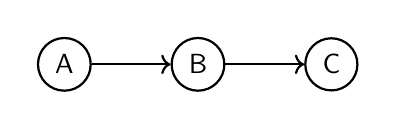
\begin{tikzpicture}
    \matrix (m) [matrix of nodes, column sep=1cm, nodes = {draw, thick, circle}] {
      A & B & C \\
    };
    \draw[thick, ->]
      (m-1-1) edge (m-1-2)
      (m-1-2) edge (m-1-3);
  \end{tikzpicture}
\end{center}

The same condition ($X_C \ind X_A \given X_B$) can also arise from the
following graph with a divergent connection. It is therefore important to note
that there can be different graphs that give the same set of independences
(formally there is an equivalence class).

\begin{center}
  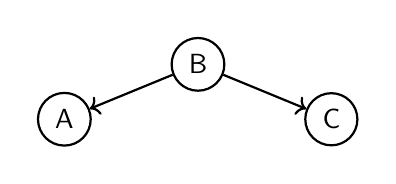
\begin{tikzpicture}
    \matrix (m) [matrix of nodes, column sep=1cm, nodes = {draw, thick, circle}] {
        & B &   \\
      A &   & C \\
    };
    \draw[thick, ->]
      (m-1-2) edge (m-2-1)
      (m-1-2) edge (m-2-3);
  \end{tikzpicture}
\end{center}

The opposite is a convergent connection, in which case both $A$ and $C$ are
parents of $B$, so there are no other non-descendent variables that can be
conditionally independent.

\begin{center}
  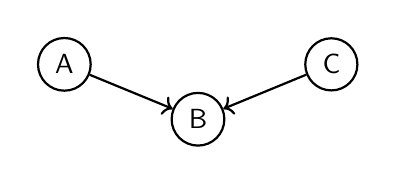
\begin{tikzpicture}
    \matrix (m) [matrix of nodes, column sep=1cm, nodes = {draw, thick, circle}] {
      A &   & C \\
        & B &   \\
    };
    \draw[thick, ->]
      (m-1-1) edge (m-2-2)
      (m-1-3) edge (m-2-2);
  \end{tikzpicture}
\end{center}

Finally a more involved example that describes the independence relations
$(X_A \ind X_E)$, $(X_B \ind X_D \given X_A, X_E)$, $(X_C \ind X_A, X_D, X_E
\given X_B)$, $(X_D \ind X_B, X_C, X_E \given X_A)$.

\begin{center}
  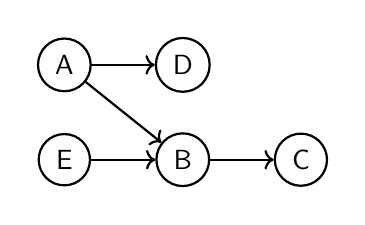
\begin{tikzpicture}
    \matrix (m) [matrix of nodes, row sep=5mm, column sep=8mm,
      nodes = {draw, thick, circle}] {
      A & D \\
      E & B & C \\
    };
    \draw[thick, ->]
      (m-1-1) edge (m-1-2)
      (m-1-1) edge (m-2-2)
      (m-2-1) edge (m-2-2)
      (m-2-2) edge (m-2-3) ;
  \end{tikzpicture}
\end{center}
The resulting expression for the joint probability is then
\begin{align*}
  p(\{\bar{X}_v\}_{v\in V}) &= 
    p(\bar{X}_A) p(\bar{X}_E) p(\bar{X}_B \given \bar{X}_A, \bar{X}_E) \\
    &\quad\cdot p(\bar{X}_C \given \bar{X}_B) p(\bar{X}_D \given \bar{X}_A).
\end{align*}

\subsection{Maximum Likelihood Estimator}

In general, given a random variable $x$ with a probability
distribution\footnote{This abuse of notation of conditioning with respect to a
non-random variable $\theta$ makes sense if you consider the ML to be a
special case of MAP.} $p(\bar{x} \given \theta)$ that depends on an unknown
parameter $\theta$, we can estimate the value of $\theta$ from observations of
$x$ using the maximum likelihood (ML) principle. Suppose we have some observations
$\{\bar{x}_i\}_{i=1}^N$ of $x$, then we define the likelihood and
log-likelihood functions to be
\begin{align*}
  L(\theta) &= \prod_{i=1}^N p(\bar{x}_i \given \theta) \text{ and}\\
  \ell(\theta) &= \log L(\theta) = \sum_{i=1}^N \log p(\bar{x}_i \given \theta)
\end{align*}
respectively. To find an estimate $\hat{\theta}$ of $\theta$ we compute
\[
  \hat{\theta} = \arg\max_\theta L(\theta) = \arg\max_\theta \ell(\theta).
\]

\subsection{Maximum A Posteriori Estimator}

With the same setup as the ML, suppose we have some prior knowledge of
$\theta$. This means that we treat $\theta$ as a random variable and there is
a known probability distribution $p_\theta(\bar{\theta})$. Then the Likelihood
function is
\[
  L(\bar{\theta}) = \prod_{i=1}^N
    p_{\theta \given x}(\bar{\theta} \given \bar{x}_i)
    = \prod_{i=1}^N \frac{
        p_{x \given \theta}(\bar{x}_i \given \bar{\theta})
        p_\theta(\bar{\theta})
      }{p_x(\bar{x}_i)},
\]
by Bayes' theorem. Then the maximum a posteriori (MAP) estimate is
\[
  \hat{\theta} = \arg \max_\theta L(\theta)
    = \arg \max_{\bar{\theta}} \prod_{i=1}^N
        p_{x \given \theta}(\bar{x}_i \given \bar{\theta})
        p_\theta(\bar{\theta}).
\]
The denominator can be ignored because it does not depend on $\theta$.


\subsection{Estimating Bayesian Networks}

If $G = (V,E)$ with $\{X_v\}_{v \in V}$ is a Bayesian network and we have some
observations $\{\bar{X}_v^i\}_{i=1}^N$ from the parametric distributions
$p_{X_v}(\bar{X}_v, \theta)$ for each $v \in V$ (fully observable, no hidden
variables), we can use the maximum likelihood estimator to estimate the
unknown $\theta$ form the observations. The likelihood function can be
decomposed into local likelihood functions using the independence relations in
$G$:
\begin{align*}
  L(\theta) &= \prod_{i=1}^N p(\{\bar{X}_v^i\}_{v \in V} \given \theta) \\
    &= \prod_{i=1}^N \prod_{v \in V}  p(
      \bar{X}_v^i \given
      \{\bar{X}_w\}_{w \in \pa(v)}, \theta) \\
    &= \prod_{v \in V} \prod_{i=1}^N
        p(\bar{X}_v^i \given \{\bar{X}_w\}_{w \in \pa(v)}, \theta) 
    = \prod_{v \in V} L_v(\theta_{v \given \pa(v)}).
\end{align*}
This decomposition can be further improved to reduce the number of
computational constraints.

If the random variables are discrete and the entire distribution is the
unknown, provided that the model is fully observable, the probabilities can be
estimated using conditional counting
\[
  p(\bar{X}_v \given \{X_w\}_{w \in \pa(v)}) \approx
    \frac{N(X_v, \pa(v))}{\sum_{u \in \pa(v)} N(X_u, \pa(u))},
\]

\todo{Fix denominator above}

\todo{explain $N$ and then MCMC}

\subsection{Network Inference}

Now suppose that we have random variables $\{X_v\}_{v \in V}$ for a set of
nodes $V$ of a directed graph $G = (V,E)$ but we do not know the structure
(its topology), that is $E$, and we would like to infer it from a set of
observations $D = \{\bar{X}_v^i\}_{v,i}$. To do so the idea is to construct a
space of candidate models and assign a score to each model, then optimize to
find the highest scoring models (this however is NP hard). The family is
constructed using prior (biological) knowledge (e.g. ``a gene as at most $n$
regulators''). For there score the \emph{Bayesian score} is defined to be
\[
  s(G) = \log p(G \given D) = \log(p(D \given G)) + \log(p(G))
\]
where the marginal likelihood is taken from a prior $\theta$
\[
  p(D \given G) = \int p(D \given G, \theta) p(\theta \given G) ~ d\theta.
\]

\begin{alg}[Greedy structure search]
  Given a set of observations $D = \{\bar{X}_v^i\}_{i,v}$ and an initial guess
  for the graph $G_0 = (V,E)$.
  \begin{algorithmic}
    \Function{greedy-search}{$G$, $D$}
      \State $\hat{G} \gets G_0$
      \Repeat
        \State $G \gets \hat{G}$
        \State \Comment{$\mathfrak{o}$ can be edge addition, removal or reversal}
        \For{each operation $\mathfrak{o}$}
          \State $G' \gets \mathfrak{o}(G)$
          \If {$G'$ is not cyclic}
            \If {$\operatorname{score}(G') > \operatorname{score}(\hat{G})$}
              \State $\hat{G} \gets G'$
            \EndIf
          \EndIf
        \EndFor
      \Until{$\hat{G} = G$}
      \State \Return $\hat{G}$
    \EndFunction
  \end{algorithmic}
\end{alg}

\subsection{Dynamic Bayesian Networks}

The model of Bayesian networks can be extended by introducing a time
dimension: let $G = (V,E)$ be a directed graph and $\{X_v(t)\}_{v\in V}$ be a
set of discrete-time stochastic processes with $t \in \{1,\ldots, T\}$ indexed
by $V$, then similar to Bayesian networks there is a factorization that
additionally involves time
\[
  p(\{X_v(t)\}_{v \in V})
    = \prod_{v \in V} \prod_{t=2}^T p(X_v(t) \given 
      \{X_u(t-1)\}_{u \in \pa(v)}).
\]

\subsection{Caveats / Challenges}

%%%%%%%%%%%%%%%%%%%%%%%%%%%%%%%%%%%%%%%%%%%%%%%%%%%%%%%%%%%%%%%%%%%%%%%%%%%%%

\section{Stoichiometric Network Analysis}

Motivated by metabolic networks the idea is to use a structural analysis from
first principles: conservation of mass (and energy) combined with
well-characterized reaction stoichiometries and reversibilities.


\subsection{Metabolic Networks}

In a metabolic network we use the vocabulary
\begin{description}
  \item[Metabolism] enzyme-catalyzed reaction;
  \item[Metabolites] educts (consumed) and products.
\end{description}
Given the reaction stoichiometry (ratios of products / educts) and reaction
directionalities (reversible or irreversible) we seek to compute metabolic
fluxes (rates of metabolic reactions). Further, we distinguish between
external and internal metabolites, so that external metabolites are assumed to
be sources / sinks.

To represent metabolic networks we use the stoichiometric matrix $N \in
\mathbb{R}^{n \times q}$, wherein on the rows there are the internal
metabolites and in the columns the reactions (incidence matrix). An element
$n_{ij}$ of $N$ is then the stoichiometric coefficient for the metabolite $i$
in reaction $j$. 

\begin{example} Consider the following metabolic network. Nodes represent
  metabolites while arrows reactions. Reversible reactions have double headed
  arrows.
  \begin{center}
    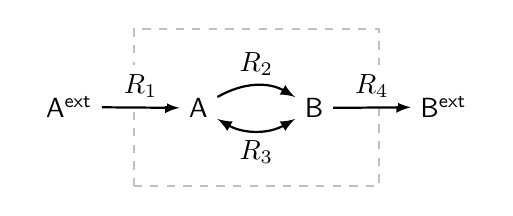
\begin{tikzpicture}
      \matrix (r) [matrix of nodes, column sep = 1cm] {
        A\textsuperscript{ext}
        & A & B & B\textsuperscript{ext} \\
      };
      \begin{scope}[thick]
        \draw[-latex] (r-1-1) -- node[above, midway, fill=white] {$R_1$} (r-1-2);
        \draw[-latex] (r-1-2) to[bend left] node[midway, above] {$R_2$} (r-1-3);
        \draw[latex-latex] (r-1-2) to[bend right] node[midway, below] {$R_3$} (r-1-3);
        \draw[-latex] (r-1-3) -- node[midway, above, fill=white] {$R_4$} (r-1-4);
      \end{scope}
      \begin{scope}[on background layer]
        \draw[thick, dashed, lightgray] ($(r-1-1)!0.5!(r-1-2) - (0,1)$)
          rectangle ($(r-1-3)!0.5!(r-1-4) + (0,1)$);
      \end{scope}
    \end{tikzpicture}
  \end{center}
  The stoichiometric matrix is
  \[
    N = \begin{bmatrix}
      1 & -1 & -1 &  0 \\
      0 &  1 &  1 & -1 \\
    \end{bmatrix}.
  \]
  Note that $R_3$ is considered only in one direction.
\end{example}

A flux distribution is a vector $r \in \mathbb{R}^q$ of reaction rates. We say
$r$ is feasible if $r_i \geq 0$ for all irreversible reactions. Then, $Nr$ is
a mass concentration $c \in \mathbb{R}^n$ so the reaction kinetics are given
by the balancing equation
\[
  \frac{dc}{dt} = N r(t) \stackrel{!}{=} 0,
\]
which we have set to zero because we are interested in knowing a quasi-steady
state. Physically this means a constant comsumption / production from the
network. Because there are more reactions that metabolites, $n \gg q$, there
is not a unique solution (underdetermined system of equations), but rather an
infinite number of them in the kernel (null space) of $N$. 

\paragraph{Linear Algebra Recap} Recall that the kernel
\[
  \ker(N) = \{ r \in \mathbb{R}^q : Nr = 0 \}
\]
has dimension $q - \rank(N)$. Recall that this subspace can be parametrized by
finding $k := q - \rank(N)$ linearly independent solutions
$\{\tilde{r}_i\}_{i=1}^k$ to the balancing equation $Nr = 0$. Then any
solution can be written as a linear combination $r = \sum_i w_i \tilde{r}_i$
for some coefficients $w_i$. If we use the $\tilde{r}_i$ as columns of a
matrix, we have the kernel matrix $K$, which by grouping the coefficients into
$w \in \mathbb{R}^k$ gives that $r = Kw$. Note that the kernel matrix is
\emph{not} unique.

\subsection{Enzyme Subsets}

The rows of the kernel matrix $K$ correspond to the reactions. If two rows of
$K$ differ only by a scalar factor, it means that the corresponding reactions
are coupled, which means that they must always operate together with a fixed
ratio in their rates. Typically (but not necessarily) this happens in linear
pathways.

\todo{slides on limitations}

\subsection{Conservation Relations}

A conservation relation describes a subset of metabolites for which a weighted
sum of their concentration is always constant in the network. In general,
conservation relations can be found by looking at the left nullspace of the
kernel matrix. That is, the weights of the conservation relations are $y \in
\mathbb{R}^n : y^\T N = 0$.

Conservation relations are especially useful to reduce the size of (ODE)
models.

\subsection{Flux Balance Analysis}

Real metabolic networks usually have a very large number of reactions, so in
practice it is impossible to solve for solution of fluxes by hand. To solve
this we incorporate additional biological knowledge by assuming again
quasi-steady state and that
\begin{enumerate}
  \item there is an \emph{objective} for instance maximize growth / energy
    (ATP) production / product yield that is calculated with $w^\T r = \sum_i
    w_i r_i$ with some coefficients $\{w_i\}_{i=1}^q$,
    
  \item for each reaction $r_i$ we (roughly) know a capacity $\alpha_i \leq
    r_i \leq \beta_i$ (e.g. for irreversible reactions $\alpha_i > 0$).
\end{enumerate}
Then we can formulate a \emph{linear program} to perform a flux balance
analysis (FBA)
\begin{align}
  \tag{FBA} \label{eqn:fba}
  \max_{r \in \mathbb{R}^q} ~ w^\T r \quad \st \quad N&r = 0 \\
       \alpha_i \leq &~r_i \leq \beta_i \nonumber
\end{align}
which can be solved using the well studied and computationally efficient
\emph{simplex method}.

\begin{example}
  \todo{Prediction of Phenotypes}
\end{example}

\begin{example}
  \todo{Prediction of Mutant behaviour}
\end{example}

\begin{example}
  \todo{evolution of metabolism}
\end{example}

\subsection{Flux Variability Analysis}

When solving the linear program for FBA, it is possible that there is not a
unique solution, but rather a set of optimal solutions (this happens when the
objective vector $w$ is perpendicular to a face of the polytope generated by
the constraints). For these case it is of interest to know how much
variability there is (for the purpose of biological analysis) between the
various solutions.

\begin{alg}[Flux Variability Analysis, FVA]
  Given the stoichiometric matrix $N$, the reactions $\{R_i\}_i$ and the
  bounds on the fluxes $\{\alpha_i\}_i, \{\beta_i\}_i$.
  \begin{algorithmic}
    \Function{FVA}{$N$, $\{R_i\}_{i=1}^q$, $\{\alpha_i\}_i, \{\beta_i\}_i$}
      \State $F \gets 0 \in \mathbb{R}^{q \times 2}$
      \For{each  $R_i$}
        \For {each direction $d \in \{1,2\}$ of $R_i$}
          \State $w \gets 0 \in \mathbb{R}^{q}$
          \State $w_i \gets (-1)^d$
          \State Solve FBA problem
            \begin{align*}
              r^\star = \max_{r \in \mathbb{R}^q} ~ w^\T r ~ \st ~ N&r = 0 \\
                \alpha_k \leq &r_k \leq \beta_k ~ \forall k
            \end{align*}
          \State $F_{i, d} \gets r^\star$
        \EndFor
      \EndFor
      \State \Return $F$
    \EndFunction
  \end{algorithmic}
\end{alg}

\subsection{Parsimonious FBA}

\subsection{Minimization of Metabolic Adjustment}

\subsection{Metabolic Pathway Analysis}

This is a different method to analyze a metabolic network which in contrast to
FBA considers all possible flux solutions using a special subset of paths
called extreme pathways. The constraints from stoichiometry define a
polyhedral cone called \emph{flux cone} when all reactions are irreversible,
and if some are not irreversible we can set the corresponding $a_i = 0$ to
define
\begin{align*}
  P(N) &= \{
    r \in \mathbb{R}^q : Nr = 0, r_i \geq 0  ~ \forall i \in \textbf{IRR}
  \} \\
  &\text{where} \quad
    \textbf{IRR} = \{ i : R_i \text{ is irreversible} \}.
\end{align*}

The flux cone $P(N)$ can be described in terms of its elementary flux modes
(EFM, mathematically they are the extreme rays of $P(N)$) $\{e^k\}_k \subset
\mathbb{R}^q$ which satisfy the following conditions
\begin{enumerate}
  \item pseudo steady state (mass conservation) $Ne^i = 0$,
  \item feasibility of reaction directions $e^i \geq 0 ~ \forall i \in \mathbf{IRR}$,
  \item elementary of reaction participations
    \[
      \forall e^k \in P(N) : R(e^k) \subset R(e^i) \Rightarrow e^k = 0 \text{ or }
      e^k \propto e^i
    \]
    where $R(e) = \{R_i : e_i \neq 0\}$ is the set of reactions involved in
    $e$.
\end{enumerate}
So, any flux distribution can be written in term of the EFMs as
$r = \sum_i \alpha_i e^i$ for some coefficients $\alpha_i \geq 0$.

\begin{example} Consider again the following simple network.
  \begin{center}
    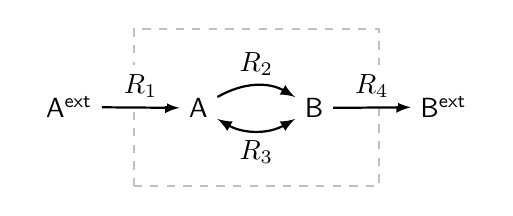
\begin{tikzpicture}
      \matrix (r) [matrix of nodes, column sep = 1cm] {
        A\textsuperscript{ext}
        & A & B & B\textsuperscript{ext} \\
      };
      \begin{scope}[thick]
        \draw[-latex] (r-1-1) -- node[above, midway, fill=white] {$R_1$} (r-1-2);
        \draw[-latex] (r-1-2) to[bend left] node[midway, above] {$R_2$} (r-1-3);
        \draw[latex-latex] (r-1-2) to[bend right] node[midway, below] {$R_3$} (r-1-3);
        \draw[-latex] (r-1-3) -- node[midway, above, fill=white] {$R_4$} (r-1-4);
      \end{scope}
      \begin{scope}[on background layer]
        \draw[thick, dashed, lightgray] ($(r-1-1)!0.5!(r-1-2) - (0,1)$)
          rectangle ($(r-1-3)!0.5!(r-1-4) + (0,1)$);
      \end{scope}
    \end{tikzpicture}
  \end{center}
  The EFMs in this case are $R(e^1) = \{R_1, R_2, R_4\}$ (above), $R(e^2) =
  \{R_1, R_3, R_4\}$ (below), $R(e^3) = \{R_2, R_3\}$ (cycle).
\end{example}

Now, the computation of the EFMs is a difficult problem, mainly because the
polyhedral description of the flux cone may contain degenerate vertices
(vertex that lies at the intersection of more than $q$ bases). One approach to
finding the EFMs is the double description method.

\todo{DD method}

\todo{applications of MPA}

\todo{caveats}

\subsection{Consortium Analysis}

The methods discussed so far do not consider interactions between species
(were only for single cells). The OptCom algorithm is a formulation of a
two-level optimization problem where individuals (cells) maximize biomass, 

\todo{OptComm}

%%%%%%%%%%%%%%%%%%%%%%%%%%%%%%%%%%%%%%%%%%%%%%%%%%%%%%%%%%%%%%%%%%%%%%%%%%%%%

\section{Dynamic Systems Fundamentals}

This section is interested in modelling biochemical reaction kinetics using
ODE models. To construct the model we use the law of mass action from reaction
kinetics:
\begin{quote}
  At constant temperature without catalyst chemical reaction rates are
  proportional to products of substrate concentrations taken to the power of
  stoichiometric coefficients (reaction order).
\end{quote}
This assumes that there is a large number of molecules and that the system is
``well-mixed'', i.e. there are no spatial heterogeneities. Hence, given a
set of $q$ reactions ($1 \leq j \leq q$) of $n$ reactants
\[
  \alpha_{1j} X_1 + \cdots + \alpha_{nj}
  \stackrel{k_j}{\longrightarrow}
  \beta_{1j} X_1 + \cdots + \beta_{nj} X_n
\]
by the law of mass action we obtain the system of ordinary differential
equations for the concentrations $c_i$ for each $X_i$
\[
  \frac{dc_i}{dt} = \sum_{j=1}^q k_j (\beta_{ij} - \alpha_{ij})
    \prod_{l=1}^n c_l^{\alpha_{lj}},
\]
The above can also be written more compactly in vector form by defining $c(t)
\in \mathbb{R}^{n}$, the (general) reaction rates $r(c(t), u(t), p)$ and using
the stoichiometric matrix $N \in \mathbb{R}^{n \times q}$
\[
  \frac{dc}{dt} = N r(c(t), u(t), p).
\]
Herein $N$ contains all $\alpha_{ij}$ and $\beta_{ij}$, while $r$ depends on
$p \in \mathbb{R}^{n_p}$ for \emph{parameters} which encapsulates all the
$k_1, \ldots, k_q$ reaction constants. In an even more general setting we will
write a model in terms of a set of ``states'' $x \in \mathbb{R}^{n_x}$
(hitherto $c$), external ``inputs'' $u(t) \in \mathbb{R}^{n_u}$ and a
``right-hand side'' of the dynamics $f(x(t), u(t), p)$, so that
\[
  \frac{dx}{dt} = f(x(t), u(t), p)
\]

\subsection{Linear Dynamics}

\todo{$\dot{x} = Ax + Bu$}

\subsection{Qualitative Analysis}

For small dimensional systems, especially 2D, we can use some qualitative
tools to analyze the system.

\begin{defn}[Nullcline]
  For a system $\frac{dx}{dt} = f(x)$, $x \in \mathbb{R}^{n_x}$, a nullcline
  is the set where the dynamics are zero in one dimension. Formally
  \[
    \left\{ x \in \mathbb{R}^{n_x} :
        \frac{dx}{dt} = \begin{bmatrix}
          f_1, \ldots, f_{k-1}, 0, f_{k+1}, \ldots, f_{n_x}
        \end{bmatrix}
    \right\}.
  \]
\end{defn}

\todo{phase space plots (portraits)}

\begin{table*}
  \caption{
    Elementary reactions.
    \label{tab:elementary-reactions}
  }
  \renewcommand\arraystretch{1.2}
  \centering
  \begin{tabular}{p{2cm} m{25mm} >{\(}l<{\)} >{\(}l<{\)} } % p{3cm}}
    \toprule
    \bfseries Name
      & \bfseries Scheme
      & \textbf{Equation}
      & \textbf{Solution} \\
      % & \bfseries Notes \\
    \midrule
    Constant Production 
      & \footnotesize \tikz{
          \node (A) {};
          \node[right=8mm of A] (B) {A};
          \draw[semithick, -latex] (A) -- node[above] {$k$} (B);
        }
      & \frac{d}{dt} \co{A} = k
      & \co{A} = \co{A}_0 + kt
      \\
    Linear Degradation
      & \footnotesize \tikz{
          \node (A) {A};
          \node[right=8mm of A] (B) {};
          \draw[semithick, -latex] (A) -- node[above] {$k$} (B);
        }
      & \frac{d}{dt} \co{A} = -k \co{A}
      & \co{A} = \co{A}_0 e^{-kt}
      \\
    Autocatalysis
      & \footnotesize \tikz{
          \node (A) {A};
          \node[right=8mm of A] (B) {};
          \draw[semithick, -latex] (A) -- node[above] {$k$} (B);
        }
      & \frac{d}{dt} \co{A} = k \co{A}
      & \co{A} = \co{A}_0 e^{kt}
      \\
    Dimerization
      & \footnotesize \tikz{
          \node (A) {A + B};
          \node[right=8mm of A] (B) {A $\cdot$ B};
          \draw[semithick, -latex] (A) -- node[above] {$k$} (B);
        }
      & \frac{d}{dt} \co{A} = \frac{d}{dt} \co{B} = k \co{A} \co{B}
      & \co{A $\cdot$ B} = k \co{A} \co{B}
      \\
    Reversible Dimerization
      & \footnotesize \tikz{
          \node (A) {A + B};
          \node[right=8mm of A] (B) {A $\cdot$ B};
          \draw[semithick, -left to] ($(A.east) + (0,.05)$) --
            node[above] {$k_1$} ($(B.west) + (0,.05)$);
          \draw[semithick, left to-] ($(A.east) - (0,.05)$) --
            node[below] {$k_{-1}$} ($(B.west) - (0,.05)$);
        }
      & \frac{d}{dt} \co{A $\cdot$ B}
        = k_1 \co{A} \co{B} - k_{-1} \co{A $\cdot$ B}
      &
      \\
    Monomolecular conversion
      & \footnotesize \tikz{
          \node (A) {A};
          \node[right=8mm of A] (B) {B};
          \draw[semithick, -latex] (A) -- node[above] {$k$} (B);
        }
      & \footnotesize 
        \frac{d}{dt} \begin{bmatrix} \co{A} \\ \co{B} \end{bmatrix}
          = k\co{A} \begin{bmatrix} -1 \\ 1 \end{bmatrix}
      & \footnotesize
        \begin{bmatrix} \co{A} \\ \co{B} \end{bmatrix}
          = \begin{bmatrix}
            \co{A}_0 e^{-kt} \\ 
            \co{B}_0 + \co{A}_0 (1 - e^{-kt})
          \end{bmatrix}
      \\
    Bimolecular conversion
      & \footnotesize \tikz{
          \node (AB) {A + B};
          \node[right=8mm of AB.east] (C) {C};
          \draw[semithick, -latex] (AB) -- node[above] {$k$} (C);
        }
      & \footnotesize
        \begin{aligned}
          \frac{d}{dt} \co{A} &= \frac{d}{dt} \co{B} = -k\co{A}\co{B} \\
          \frac{d}{dt} \co{C} &= k \co{A} \co{B}
        \end{aligned}
        % \frac{d}{dt} \begin{bmatrix}
        %   \co{A} \\ \co{B} \\ \co{C}
        % \end{bmatrix}
        % = k\co{A}\co{B} \begin{bmatrix}
        %     -1 \\ -1 \\ 1
        % \end{bmatrix}
      \\
    \bottomrule
  \end{tabular}
\end{table*}

\subsection{Michaelis-Menten Enzyme Kinetics}

To model an enzymatic reaction from a substrate S to a product P we will
assume the following reaction

\begin{center}
  \schemestart
    E + S \arrow{<=>[$k_1$][$k_{-1}$]}
    E $\cdot$ S \arrow{<=>[$k_2$][$k_{-2}$]}
    E + P
  \schemestop
\end{center}
And then we will make the following assumptions
\begin{enumerate}
  \item There is no feedback by the product, so $k_{-2} = 0$.
  \item There is a constant total quantity (concentration) of enzyme $\co{E}^t
    = \co{E} + \co{E $\cdot$ S}$. This reduces the number of variables in the
    ODE model.
  \item The reaction is in quasi steady-state because of time-scale separation
    ($k_1, k_{-1} \gg k_2$) which means that $\frac{d}{dt} \co{E $\cdot$ S}
    \approx 0$.
  \item There is an excess of substrate over the enzyme, so $\co{S} \approx
    \co{S}_0$ is a constant, making $\frac{d}{dt} \co{S} = 0$ (e.g. justified
    in metabolic networks).
\end{enumerate}
When applied to an ODE model of the first reaction these assumptions will lead
to the following system of algebraic equations
\begin{align*}
  0 &= -k_1 \co{E}^t \co{S}_0
    + (k_1 \co{S}_0 + k_{-1}) \co{E $\cdot$ S} \\
  0 &= k_1 \co{E}^t \co{S}_0 - (k_1 \co{S}_0 + k_{-1} + k_2) \co{E $\cdot$ S}
\end{align*}
that can be solved for $\co{S $\cdot$ E}$ yielding
\[
  \co{S $\cdot$ E} = \frac{
    \co{S}_0 \co{E}^t
  }{
    \co{S}_0 + \frac{k_2 + k_{-1}}{k_1}
  }
\]
Then, inserted this result into the next reaction model gives
\[
  \frac{d\co{P}}{dt} = k_2 \co{S $\cdot$ E} = \frac{
    k_2 \co{S}_0 \co{E}^t
  }{
    \co{S}_0 + \frac{k_2 + k_{-1}}{k_1}
  }
  = \nu,
\]
wherein since everything on the left hand side is constant we defined $\nu$
to be the so-called reaction velocity, which itself is described by two
parameters
\[
  \nu = \frac{\nu_\text{max} \co{S}_0}{\co{S}_0 + K_M},
\]
the maximal reaction rate $\nu_\text{max}$ and the Michaelis-Menten constant
$K_M$. The latter can be understood as a measure for the affinity between the
enzyme and the substrate. Physically, it is the substrate concentration at
half of the maximal rate.

\paragraph{Applicability} Note that the presently derived Michaelis-Mensen
dynamics only apply for quasi steady state concentrations (timescale $1$ to
$40$ s). Outside of this range it is an ``initial phase`` ($t < 0.9$ s)
and substrate depletion ($t > 30$ s).

\subsubsection{Competitive Inhibition}

For competitive inhibition we assume the reaction
\begin{center}
  \schemestart
    E + S \arrow{<=>[$k_1$][$k_{-1}$]}
    E $\cdot$ S \arrow{<=>[$k_2$][$k_{-2}$]}
    E + P
  \schemestop
  \medskip\newline
  \schemestart
    E + I \arrow{<=>[$k_3$][$k_{-3}$]} E $\cdot$ I
  \schemestop
\end{center}
and further assume
\begin{enumerate}
  \item The inhibitor is also conserved.
  \item Quasi steady-state for enzyme complexes.
\end{enumerate}
Then, by going through the same process as before to solve for the
concentrations will result in
\[
  \nu = \frac{
    k_2 \co{S}_0 \co{E}^t
  }{
    \co{S}_0 + \frac{k_2 + k_{-1}}{k_1} \left(
      1 + \frac{k_3 \co{I}}{k_{-3}}
    \right)
  }
  = \frac{\nu_\text{max} \co{S}_0}{\co{S}_0 + K_M \left(
      1 + \frac{\co{I}}{K_I} \right)}
\]
wherein we introduce an inhibition constant $K_I$. Put into words, the
competitive inhibitor reduces the apparent substrate affinity.

\subsubsection{Non-Competitive Inhibition}

If we instead assume the following reaction scheme
\begin{center}
  \schemestart
    E + S \arrow(eps -- eds){<=>[$k_1$][$k_{-1}$]}
    E $\cdot$ S \arrow(eds -- epp){<=>[$k_2$][$k_{-2}$]}
    E + P
    \arrow(@eps --){<=>[$k_3$][$k_{-3}$]}[-90]
    E $\cdot$ I \arrow(-- epips){<=>[$k_4$][$k_{-4}$]}
    E $\cdot$ I $\cdot$ S \arrow(-- epips){<=>[$k_5$][$k_{-5}$]}[90]
  \schemestop
\end{center}
then the resulting velocity (assuming again quasi steady-state for complexes
and inhibitor conservation) will be
\[
  \nu =
  \frac{\nu_\text{max} \co{S}_0}{\co{S}_0 + K_M}
  \left( 1 + \frac{\co{I}}{K_I} \right)^{-1},
\]
for a new constant $K_I$  that depends on $k_1, k_2, \ldots, k_{-5}$.
Hence, non-competitive inhibition will reduce the maximal reaction velocity.

\subsubsection{Cooperativity}

The converse of the previous section is cooperativity, whereby usually a large
assembly of enzymes are spatially close together and acts as an integrated
metabolic factory. In this case instead of considering each enzyme in the
chain we simplify the model by creating an artificial reaction that requires
$n$ substrate molecules to produce $n$ products
\begin{center}
  \schemestart
    E + $n$S \arrow{<=>[$k_1$][$k_{-1}$]}
    E $\cdot$ $n$S \arrow{<=>[$k_2$][$k_{-2}$]}
    E + $n$P
  \schemestop
\end{center}
This results in the rate law
\[
  \nu = \frac{\nu_\text{max} \co{S}_0^n}{\co{S}_0^n + K_M^n}
\]
and we call $n$ the Hill coefficient. Increasing the Hill coefficient will
change the signal response characteristic from hyperbolic (`graded') to
sigmoidal (`ultrasensitive').

\subsection{Feedback Mechanisms}

To model more complex (biological) systems such as ones showing oscillatory
behaviour we need to analyze further the notion of feedback, that is,
circular patterns of interactions (see Fig. \ref{fig:feedback}).

\begin{figure}
  \centering
  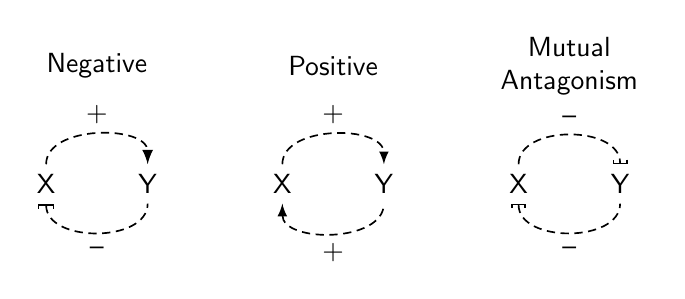
\begin{tikzpicture}[semithick, densely dashed]
    \begin{scope}
      \node (X) {X};
      \node[right = 8mm of X] (Y) {Y};
      \draw[-latex] (X) to[out=90, in=90, thick]
        node[midway, above] {+} (Y);
      \draw[Bracket-] (X) to[out=-90, in=-90, thick] 
        node[midway, below] {--} (Y);
      \coordinate (A) at ($(X)!0.5!(Y) + (0,15mm)$);
    \end{scope}

    \begin{scope}[xshift=3cm]
      \node (X) {X};
      \node[right = 8mm of X] (Y) {Y};
      \draw[semithick, -latex] (X) to[out=90, in=90, thick] 
        node[midway, above] {+} (Y);
      \draw[semithick, latex-] (X) to[out=-90, in=-90, thick]
        node[midway, below] {+} (Y);
      \coordinate (B) at ($(X)!0.5!(Y) + (0,15mm)$);
    \end{scope}

    \begin{scope}[xshift=6cm]
      \node (X) {X};
      \node[right = 8mm of X] (Y) {Y};
      \draw[semithick, -Bracket] (X) to[out=90, in=90, thick]
        node[midway, above] {--} (Y);
      \draw[semithick, Bracket-] (X) to[out=-90, in=-90, thick]
        node[midway, below] {--} (Y);
      \coordinate (C) at ($(X)!0.5!(Y) + (0,15mm)$);
    \end{scope}

    \node at (A) {Negative};
    \node at (B) {Positive};
    \node[text width = 2cm, align = center] at (C) {Mutual \\ Antagonism};
  \end{tikzpicture}
  \caption{Feedback types. \label{fig:feedback}}
\end{figure}

\begin{example} Consider the production-degradation dynamics
  \[
    \frac{d\co{A}}{dt} = k_1 u - k_2 \co{A}
    \quad \Rightarrow \quad
    \co{A} = \frac{k_1 u}{k_2} (1 - e^{-k_2 t})
  \]
  with the following reaction scheme.
  \begin{center}
    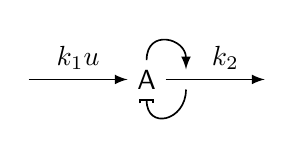
\begin{tikzpicture}
      \node (A) {A};
      \draw[semithick, -latex] (A) ++(-1.5,0) -- node[midway, above] {$k_1 u$} (A);
      \draw[semithick, -latex] (A) -- ++(.5,0) node (F) {} 
        -- node[midway, above] {$k_2$} ++(1,0);
      \draw[semithick, -latex] (A) to[out=90, in=90, looseness=2] (F);
      \draw[semithick, Bracket-] (A) to[out=-90, in=-90, looseness=2] (F);
    \end{tikzpicture}
  \end{center}

  An increase in the production of A also accelerates the degradation of A,
  which reduces the concentration of A (negative feedback). From the analytic
  solution we can see that after a perturbation (with $u$) the system will
  return to a steady state (homeostasis).
\end{example}

\begin{example}
  Consider the more complex reaction scheme below, where protein X is a
  phosphatase that dephosphorylates Y\textsubscript{p}, and the
  dephosphorylated from Y activates a degradation of X (negative feedback).
  \begin{center}
    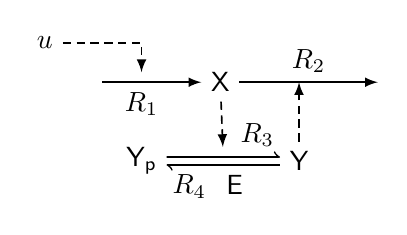
\begin{tikzpicture}
      \node (X) {X};
      \node[yshift = -10mm, xshift = -10mm] (Yp) {Y\textsubscript{p}};
      \node[yshift = -10mm, xshift =  10mm] (Y) {Y};
      
      \begin{scope}[semithick]
        \draw[-latex] (X) ++ (-15mm,0) -- ++(5mm,0)
          node (Fu) {} node[below] {$R_1$} -- (X);

        \draw[-latex] (X) -- node[midway, above] {$R_2$} ++(2,0)
          coordinate (FY);

        \draw[-left to] ($(Yp.east)+(0,.05)$) -- 
          ($(Yp.east)!0.5!(Y.west) + (0,.05)$) node (FX) {}
          -- 
          node[pos=.6, above] {$R_3$} 
          ($(Y.west)+(0,.05)$);

        \draw[left to-] ($(Yp.east)-(0,.05)$) -- 
          node[pos = .6, below] {E}
          node[pos = .2, below] {$R_4$} ($(Y.west)-(0,.05)$);

        \begin{scope}[densely dashed]
          \draw[-latex] (X) -- (FX);
          \draw[-latex] (Y) -- (FY -| Y);
          \draw[-latex] (Fu) ++(-1, 5mm)
            node[left] {$u$} -| (Fu);
        \end{scope}
    \end{scope}
    \end{tikzpicture}
  \end{center}
  The system is described by the two state ODE model with Michaelis-Menten
  kinetics
  \begin{align*}
    \frac{d\co{X}}{dt} &= k_1 u - k_2 \co{Y} \co{X}, \\
    \frac{d\co{Y}}{dt} &= \frac{
      k_3\co{X}(\co{Y}^t - \co{Y})
    }{
      K_{M,3} + \co{Y}^t + \co{Y}
    }
    - \frac{
      k_4 \co{E} \co{Y}
    }{
      k_{M,4} + \co{Y}
    }.
  \end{align*}
  To find the steady state solutions for this system we can compute the
  nullclines by setting the derivatives to zero. For convenience we introduce
  some new scaled variables
  \begin{align*}
    y &= \frac{\co{Y}}{\co{Y}^t},
      & \nu_1 &= k_3 \co{X},
      & \nu_2 &= k_4 \co{E}, \\
    J_1 &= \frac{K_{M,3}}{\co{Y}^t},
      & J_2 &= \frac{K_{M,4}}{\co{Y}^t},
  \end{align*}
  so that the scaled nullcline for $\co{Y}$ is
  \[
    \nu_1 (1 - y) (J_2 + y) = \nu_2 y (J_1 + 1 - y),
  \]
  which can be solved analytically and the solution
  \begin{align*}
    y &= \frac{
      2\nu_1 J_2
    }{
      B + \sqrt{B^2 - 4 (\nu_2 - \nu_1) \nu_1 J_2}
    } =: G(\nu_1, \nu_2, J_1, J_2) \\
    &\text{where } B = \nu_2 - \nu_1 + \nu_2 J_1 + \nu_1 J_2
  \end{align*}
  is known as the Goldbeter-Koshland function. This solution is sigmoidal-like
  in the input $\co{X}$ (switch-like).
\end{example}


\begin{example}
  We now consider the following reaction scheme which is a system with a
  positive feedback.
  \begin{center}
    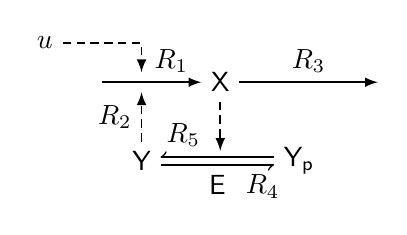
\begin{tikzpicture}
      \node (X) {X};
      \node[yshift = -10mm, xshift = -10mm] (Y) {Y};
      \node[yshift = -10mm, xshift =  10mm] (Yp) {Y\textsubscript{p}};
      
      \begin{scope}[semithick]
        \draw[-latex] (X) ++ (-15mm,0) -- ++(5mm,0)
          node (FX) {} -- node[midway, above] {$R_1$} (X);

        \draw[-latex] (X) -- node[midway, above] {$R_3$} ++(2,0);

        \draw[right to-] ($(Y.east)+(0,.05)$) -- 
          node[pos = .2, above] {$R_5$} ($(Yp.west)+(0,.05)$);

        \draw[-right to] ($(Y.east)-(0,.05)$) -- 
          node[midway, below] {E}
          node[pos=.9, below] {$R_4$} ($(Yp.west)-(0,.05)$);

        \node (FXp) at (FX -| Y) {};
        \node (FYp) at (Y -| X) {};

        \begin{scope}[densely dashed]
          \draw[-latex] (X) -- (FYp);
          \draw[-latex] (Y) -- node[midway, left] {$R_2$} (FXp);
          \draw[-latex] (FXp) ++(-1, 5mm) node[left] {$u$} -| (FXp);
        \end{scope}
      \end{scope}
    \end{tikzpicture}
  \end{center}
  Using Michealis-Menten kinetics the dynamics are
  \begin{align*}
    \frac{d\co{X}}{dt} &= k_1 u + k_2 \co{Y} - k_3 \co{X}, \\
    \frac{d\co{Y}}{dt} &= \frac{
      k_4 \co{X} (\co{Y}^t - \co{Y})
    }{
      K_{M,4} + \co{Y}^t - \co{Y}
    }
    - \frac{
      k_5 \co{E} \co{Y}
    }{
      K_{M,5} \co{Y}
    }.
  \end{align*}
  Intersecting the nullclines we get the steady state concentrations
  \begin{align*}
    \co{Y} &= \frac{k_3 \co{X} - k_1 u}{k_2}, \\
    \co{Y} &= \co{Y}^t G\left(
      k_4 \co{X}, k_5 \co{E}, \frac{K_{M,4}}{\co{Y}^t}, \frac{K_{M,5}}{\co{Y}^t}
    \right).
  \end{align*}
  This system can have up to two stable steady states and an unstable steady
  state.
\end{example}

% Add phase portraits
% \begin{figure}
%   \begin{tikzpicture}
%     \begin{axis}
%     \end{axis}
%   \end{tikzpicture}
% \end{figure}

\begin{example} Finally consider this the reaction scheme below which exhibits
  mutual antagonism.
  \begin{center}
    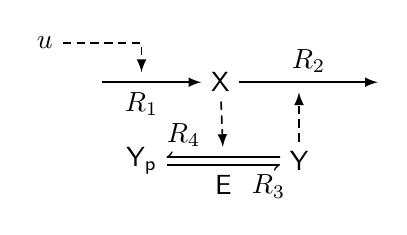
\begin{tikzpicture}
      \node (X) {X};
      \node[yshift = -10mm, xshift = -10mm] (Yp) {Y\textsubscript{p}};
      \node[yshift = -10mm, xshift =  10mm] (Y) {Y};
      
      \begin{scope}[semithick]
        \draw[-latex] (X) ++ (-15mm,0) -- ++(5mm,0)
          node (Fu) {} node[below] {$R_1$} -- (X);

        \draw[-latex] (X) -- node[midway, above] {$R_2$} ++(2,0)
          coordinate (FY);

        \draw[right to-] ($(Yp.east)+(0,.05)$) -- 
          ($(Yp.east)!0.5!(Y.west) + (0,.05)$) node (FX) {}
          node[pos=.3, above] {$R_4$} -- 
          ($(Y.west)+(0,.05)$);

        \draw[-right to] ($(Yp.east)-(0,.05)$) -- 
          node[pos = .5, below] {E}
          node[pos = .9, below] {$R_3$} ($(Y.west)-(0,.05)$);

        \node (FXd) at (FY -| Y) {};

        \begin{scope}[densely dashed]
          \draw[-latex] (X) -- (FX);
          \draw[-latex] (Y) -- (FXd);
          \draw[-latex] (Fu) ++(-1, 5mm) node[left] {$u$} -| (Fu);
        \end{scope}
    \end{scope}
    \end{tikzpicture}
  \end{center}
  Here the dynamics are
  \begin{align*}
    \frac{d\co{X}}{dt} &= k_1 u - (k_2' + k_2 \co{Y}) \co{X}, \\
    \frac{d\co{Y}}{dt} &= \frac{
      k_2 \co{E} (\co{Y}^t - \co{Y})
    }{
      K_{M,3} + \co{Y}^t - \co{Y}
    }
    - \frac{k_4 \co{X}\co{Y}}{K_{M,4} + \co{Y}},
  \end{align*}
  and the nullclines
  \begin{align*}
    \co{Y} &= \frac{k_1 u - k_2' \co{X}}{k_2 \co{X}}, \\
    \co{Y} &= \co{Y}^t G\left(
      k_3 \co{E}, k_4 \co{X},
      \frac{K_{M,3}}{\co{Y}^t},
      \frac{K_{M,4}}{\co{Y}^t}
    \right).
  \end{align*}
  \todo{mention switch}
\end{example}

\todo{phase portraits and bifurcation diagrams}

\subsection{Bifurcations}

In both the negative and positive feedback examples we had the freedom to
choose $u$. By varying $u$ the number of steady states changes, and so the
system can have qualitatively different behaviours. When by changing $u$ the
number of steady states (aka attractors) changes, we say that the value of $u$
at that point is \emph{critical}, and there is a \emph{bifurcation}. If we
plot the steady states as a function of $u$ we call it a \emph{bifurcation
diagram}.

\todo{Add a bifurcation diagram}

\subsection{Oscillators}

\begin{example}[Activator-Inhibitor]
  Consider the following reaction scheme, where again protein X is a
  phosphatase that dephosphorylates Y\textsubscript{p}, protein Y actvates a
  production of X (positive feedback on X) and now additionally a protein Z
  whose production is mediated by Y activates a degradation of X (negative
  feedback on X).
  \begin{center}
    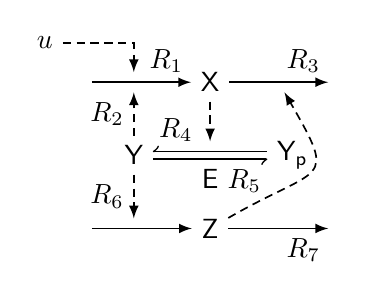
\begin{tikzpicture}
      \matrix (m) [
        row sep = 4mm, column sep = 5mm,
      ] {
                       & \node (X) {X}; \\
        \node (Y) {Y}; &                 & \node (Yp) {Y\textsubscript{p}}; \\
                       & \node (Z) {Z}; \\
      };

      % production of X
      \draw[semithick, -latex] (X) ++(-15mm,0) --
        node[midway] (FX) {}
        node[near end, above] {$R_1$} (X);

      % degradation of X
      \draw[semithick, -latex] (X) --
        node[midway] (FXd) {}
        node[near end, above] {$R_3$} ++(15mm,0);

      \draw[semithick, right to-] ($(Y.east)+(0,.05)$) --
        node[midway] (FY) {}
        node[pos=.2, above] {$R_4$}
        ($(Yp.west)+(0,.05)$);

      \draw[semithick, -right to] ($(Y.east)-(0,.05)$) --
        node[midway, below] {E} 
        node[pos=.8, below] {$R_5$}
        ($(Yp.west)-(0,.05)$);

      \begin{scope}[semithick]
        \draw[-latex] (Z) ++(-15mm,0) -- node[midway] (FZ) {} (Z);
        \draw[-latex] (Z) -- node[near end, below] {$R_7$} ++(15mm,0);

        \node (FXp) at (FX -| Y) {};
        \node (FYpp) at (FY -| X) {};
        \node (FZp) at (FZ -| Y) {};

        \begin{scope}[densely dashed]
          \draw[-latex] (Y) -- node[midway, left] {$R_2$} (FXp);
          \draw[-latex] (Y) -- node[midway, left] {$R_6$} (FZp);
          \draw[-latex] (X) -- (FYpp);

          \draw[-latex] (FX) ++(-10mm, 5mm) node[left] {$u$} -| (FXp);
          \draw[-latex] (Z) to[out=30, in=-60, looseness=2] (FXd);
        \end{scope}
      \end{scope}
    \end{tikzpicture}
  \end{center}
  To analyze the dynamics we assume steady-state for the interconversion
  between Y and Y\textsubscript{p}. So we have
  \begin{equation} \label{eqn:osc-y-yp-ss}
    \co{Y} = \co{Y}^t G\left(
      k_4 \co{X}, k_5 \co{E}, \frac{K_{M,4}}{\co{Y}^t}, \frac{K_{M,5}}{\co{Y}^t}
    \right).
  \end{equation}
  The other two concentrations have the model
  \begin{align*}
    \frac{d\co{X}}{dt} &= k_1 u + k_2 \co{Y} - k_3 \co{Z} \co{X}, \\
    \frac{d\co{Z}}{dt} &= k_6 \co{Y} - k_7 \co{Z},
  \end{align*}
  and their respective nullclines are given by
  \begin{align*}
    \co{Z} &= \frac{k_1 u + k_2 \co{Y}}{k_2 \co{X}}, &
    \co{Z} &= \frac{k_6}{k_7} \co{Y}.
  \end{align*}

  The bifurcation diagram for this system in the steady state concentration of
  X has two critical values $u_{c,1}$ and $u_{c,2}$. The dynamics of $\co{X}$
  are stable for $u < u_{c,1}$ and $u_{c,2} < u$, while unstable for $u \in
  (u_{c,1}, u_{c,2})$. In the unstable region is a \emph{limit cycle}, and the
  concentration of X oscillates.
\end{example}

Another example is the motif of substrate-depletion oscillator, which in
biology comes up in glycolitic oscillations, cell cycle control, calcium
signaling and predator-prey interactions (in ecosystems).

\begin{example}[Substrate-Depletion]
  Consider the substrate depletion system with the reaction scheme below. The
  metabolite X converts to Z, which in terms is a regulator of formation of Y
  (from Y\textsubscript{p}). Then because the dephosphorylated form of protein
  Y catalyzes the conversion of X this is a negative feedback.
  \begin{center}
    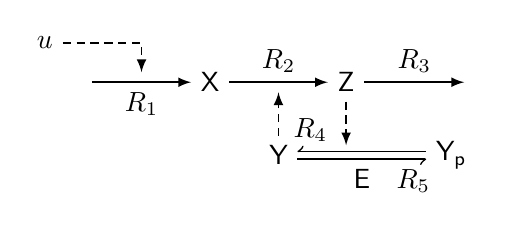
\begin{tikzpicture}
      \matrix [row sep = 4mm, column sep = 4mm] {
        \node (X) {X}; & & \node (Z) {Z}; \\
        & \node (Y) {Y}; & & & \node (Yp) {Y\textsubscript{p}}; \\
      };

      \begin{scope}[semithick]
        \draw[-latex] (X) ++(-15mm,0) --
          node[midway] (FXp) {} 
          node[midway, below] {$R_1$} (X);

        \draw[-latex] (X) -- 
          node[midway] (FZ) {}
          node[midway, above] {$R_2$} (Z);
        \draw[-latex] (Z) -- node[midway, above] {$R_3$} ++(15mm, 0);
        
        \draw[right to-] ($(Y.east)+(0,.05)$) --
          node[pos=.1, above] {$R_4$} ($(Yp.west)+(0,.05)$);

        \draw[-right to] ($(Y.east)-(0,.05)$) -- 
          node[midway, below] {E}
          node[pos=.9, below] {$R_5$} ($(Yp.west)-(0,.05)$);

          \node (FZp) at (FZ -| Y) {};
          \node (FYpp) at (Y -| Z) {};

          \begin{scope}[densely dashed]
            \draw[-latex] (Y) -- (FZp);
            \draw[-latex] (Z) -- (FYpp);
            \draw[-latex] (FXp) ++(-10mm, 5mm) node[left] {$u$} -| (FXp);
          \end{scope}
      \end{scope}
    \end{tikzpicture}
  \end{center}
  Again we assume a steady state for the reactions between Y and
  Y\textsubscript{p}, and thus we have again equation \eqref{eqn:osc-y-yp-ss},
  but with Z instead of X
  \[
    \co{Y} = \co{Y}^t G\left(
      k_4 \co{Z}, k_5 \co{E},
      \frac{k_{M,4}}{\co{Y}^t},
      \frac{k_{M,5}}{\co{Y}^t}
    \right).
  \]
  The other equations are
  \begin{align*}
    \frac{d\co{X}}{dt} &= k_1 u - (k_2' + k_2 \co{Y}) \co{X}, \\
    \frac{d\co{Z}}{dt} &= (k_2' + k_2 \co{Y}) \co{X} - k_3 \co{Z},
  \end{align*}
  and the nullclines
  \begin{align*}
    \co{X} &= \frac{k_1 u}{k_2' + k_2 \co{Y}}, &
    \co{X} &= \frac{k_3 \co{Z}}{k_2' + k_2 \co{Y}}.
  \end{align*}
  Similarly to the activator-inhibitor dynamics these dynamics also present an
  oscillating limit cycle for certain values of $u$.
\end{example}

\subsection{Linearization for Stability Analysis}

\todo{Linearization}

\begin{example}[Simplified Substrate Depletion]
  We consider again the substrate depletion system but assuming a low
  concentration of Z we approximate the Goldbeter-Koshland
  function with a parabola for the steady state of Y
  \[
    G(\nu_1)
    \approx 
    \frac{\partial^2 G}{\partial \nu_1^2}(\bar{\nu}_1) \nu_1^2 
      + \frac{\partial G}{\partial \nu_1}(\bar{\nu}_1) \nu_1,
  \]
  with the following reaction scheme.
  \begin{center}
    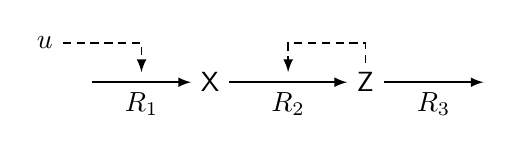
\begin{tikzpicture}
      \node (X) {X};
      \node[right = 15mm of X] (Z) {Z};

      \begin{scope}[semithick]
        \draw[-latex] (X) ++ (-15mm, 0) -- 
          node[midway, below] {$R_1$}
          node[midway] (FXp) {} (X);
        \draw[-latex] (X) --
          node[midway, below] {$R_2$}
          node[midway] (FZp) {} (Z);
        \draw[-latex] (Z) -- node[midway, below] {$R_3$} ++(15mm, 0);
        \begin{scope}[densely dashed]
          \draw[-latex] (FXp) ++ (-10mm, 5mm) node[left] {$u$} -| (FXp);
          \draw[-latex] (Z) |- ++(0, 5mm) -| (FZp);
        \end{scope}
      \end{scope}
    \end{tikzpicture}
  \end{center}
  For the sake of exposure we choose unitary kinetic rates (except $k_1 := k$)
  and $\bar{\nu}_1$ such that the dynamics simplify down to
  \[
    \frac{dx}{dt} = 
    \frac{d}{dt} \begin{bmatrix} \co{X} \\ \co{Z} \end{bmatrix}
    = \begin{bmatrix}
      u - (k + \co{Z}^2) \co{X} \\
      (k + \co{Z}^2) \co{X} - \co{Z}
    \end{bmatrix}
    = f(x, u).
  \]
  Then to analyze its stability, we look at the state transition matrix of the
  dynamics linearized at the steady state
  \begin{align*}
    J_{ss} :=
    \frac{\partial f}{\partial x} \bigg|_{x_{ss}}
    = \begin{bmatrix}
      - (k + u^2) & \dfrac{-2u}{k + u^2} \\
      k + u^2 & \dfrac{u^2 - k}{k + u^2}
    \end{bmatrix},
  \end{align*}
  where
  \[
    f(x_{ss}, u) = 0 
    \quad \Rightarrow \quad 
    x_{ss} = \begin{bmatrix}
      \dfrac{u}{k + u^2} &
      u
    \end{bmatrix}^\T,
  \]
  which has eigenvalues
  \begin{align*}
    \lambda &= \frac{1}{2} \left[
      \tr (J_{ss}) + \sqrt{
        \tr (J_{ss})^2 - 4 \det (J_{ss})
      }
    \right].
  \end{align*}

  \todo{2D bifurcation diagram}
\end{example}

%%%%%%%%%%%%%%%%%%%%%%%%%%%%%%%%%%%%%%%%%%%%%%%%%%%%%%%%%%%%%%%%%%%%%%%%%%%%%

\section{System Identification}

We consider an ODE model ($x \in \mathbb{R}^{n_x}, u \in \mathbb{R}^{n_u}$)
containing a parameter vector $p \in \mathbb{R}^{n_p}$ given by
\begin{equation} \label{eqn:dynamics-p}
  \frac{dx}{dt} = f(x(t), u(t), p),
\end{equation}
which has a (generally unknown) solution
\begin{equation} \label{eqn:sol-p}
  x(t, p) = x(0) + \int_0^t f(x(s, p), u(s), p) ~ ds
\end{equation}
We denote by $p^\star$ the optimal set of parameters, that is, those that
bring the model closest to reality. The goal of this section is to find
$p^\star$.

\subsection{Measurements}

Hereinafter we suppose we have $N$ field measurements $\{x_i\}_{i=1}^N$ taken
at discrete time intervals $\{t_i\}_{i=1}^N$. We assume that the measured
values are given by the true value corrupted by i.i.d zero-mean Gaussian noise
with covariance $\Sigma_\epsilon$, i.e.
\begin{equation} \label{eqn:measurement-model}
  x_i = x(t_i, p^\star) + \epsilon_i, \quad i = 1, \ldots, N
\end{equation}
where  $\epsilon_i \sim \mathcal{N}(0, \Sigma_\epsilon)$. Then we define the
identification error $e_i = x(t_i, p) - x_i$ for our estimate of $p$ and
functional that is to be minimized
\[
  \phi(p) = \frac{1}{2} \sum_{i=1}^N e_i^\T Q e_i
\]
with a (positive semidefinite) weighting matrix $Q$. For instance if $Q = I$
all errors are weighted equally. In reality since our measurements have a
certain uncertainty (stemming from the tools we are using) it is more common
to set $Q$ to be the inverse of the covariance matrix of the measurement noise
$Q = \Sigma_\epsilon^{-1}$.

An alternative identification error functional $\phi$ could be constructed
from potential energy surfaces (variation of the potential energy, enthalpy,
as a function of the conformation), since thermodynamically the most frequent
configurations lie at the global free energy minimum. In this case however
there are usually multiple minima and it is not easy to find the global
minimum.

\subsection{Sensitivity}

Because of the dynamics, the influence of each parameter on the model may
change over time and the \emph{sensitivity function} quantifies this exactly.
Formally if we consider an initial set of parameters $\bar{p}$ the sensitivity
over time is defined\footnote{We can also consider the sensitivity to be a
function of $p$, so $S(t, p)$ is a function that shows how the parameters
deviate from an initial value $p$ after some time $t$.} to be
\[
  S(t) = \frac{\partial x(t, p)}{\partial p} \bigg|_{\bar{p}},
  \quad S: \mathbb{R} \to \mathbb{R}^{n_p \times n_x}.
\]
However since we don't know $x(t, p)$, to compute $S(t)$ we use the
differential sensitivity equation. To derive it we proceed by inserting
\eqref{eqn:sol-p} in $S(t)$ which gives
\begin{align*}
  S(t) &= \frac{\partial}{\partial p} \int_0^t f(x(s, p), u(s), p) ~ ds \\
  &= \int_0^t \frac{\partial f}{\partial x} \frac{\partial x}{\partial p}
   + \frac{\partial f}{\partial p} ~ ds
    = \int_0^t \frac{\partial f}{\partial x} S(s)
      + \frac{\partial f}{\partial p} ~ ds
\end{align*}
then we remove the integral by differentiating with respect to time to obtain
to obtain the differential equation
\[
  \frac{dS}{dt} = \frac{\partial f}{\partial x} \bigg|_{\bar{p}} S(t)
    + \frac{\partial f}{\partial p} \bigg|_{\bar{p}}, \quad S(0) = 0.
\]
This equation can be (numerically) solved for $S(t)$. Since the ODE model is
usually also solved numerically, it is common to directly solve the augmented
system
\[
  \dot{\xi} =
  \begin{bmatrix} \dot{x} \\ \dot{S} \end{bmatrix} =
  \underbrace{\begin{bmatrix}
    f(x, u, p) \\
    \frac{\partial f}{\partial x} \big|_{\bar{p}} S
    + \frac{\partial f}{\partial t} \big|_{\bar{p}}
  \end{bmatrix}}_{\tilde{f}(\xi, u, p)},
  \quad \xi(0) = \begin{bmatrix}
    x(0) \\ 0
  \end{bmatrix}.
\]

\subsection{Gradient-based Methods}

To find $p^\star$ for \eqref{eqn:dynamics-p} we want to minimize the error
$\phi(p)$ that is generally non-linear in $p$, and to do so we use Newton's
method. To start we use an initial guess for the parameters $p_0$, then we
iteratively apply steps $s_0, s_1, \ldots$ as $p_{k+1} = p_k + s_k$ to reach
(get close to) $p^\star$. At each iteration we use a second order
approximation
\[
  \phi(p_{k+1}) = \phi(p_k + s_k) \approx \phi(p_k)
    + \frac{\partial \phi}{\partial p} \bigg|_{p_k} s_k
    + \frac{1}{2} s_k^\T \frac{\partial^2 \phi}{\partial p^2} s_k
\]
and then we choose $s_k$ such that the above is minimized by solving
\[
  \frac{\partial^2 \phi}{\partial p^2} \bigg|_{p_k} s_k
    = - \frac{\partial \phi}{\partial p} \bigg|_{p_k}.
\]
The iteration is halted when the quantity $\|\phi(p_{k+1}) - \phi(p_k)\|$
becomes small enough.

Newton's method as just described does not make use of the statistical
information we know about our measurements. To incorporate statistical
information we compute how of the structure of the Hessian of $\phi$ is
related to $S(t)$:
\begin{align*}
  \frac{\partial^2 \phi}{\partial p^2}
    &= \frac{\partial^2}{\partial p^2} \left\{
        \frac{1}{2} \sum_{i=1}^N [x(t_i, p) - x_i]^\T Q [x(t_i, p) - x_i]
      \right\} \\
    &= \sum_{i=1}^N \frac{\partial}{\partial p} \left\{
        [x(t_i, p) - x_i]^\T Q \frac{\partial x}{\partial p}
      \right\} \\
    &= \sum_{i=1}^N \frac{\partial x}{\partial p}^\T Q
      \frac{\partial x}{\partial p} + x(t_i, p) Q\frac{\partial^2 p}{\partial p^2}
      - x_i Q \frac{\partial^2 x}{\partial p^2} \\
    &= \sum_{i=1}^N S(t_i)^\T Q S(t_i)
      + e_i Q \frac{\partial^2 x}{\partial p^2}.
\end{align*}
Now, if we take the expectation, since the error is zero-mean (assume unbiased
estimator $p$ of $p^\star$)
\[
  \E{\frac{\partial^2 \phi}{\partial p^2}} = \sum_{i=1}^N S(t_i)^\T Q S(t_i),
\]
and in particular if we replace $Q$ with inverse of the measurement error
covariance matrix $\Sigma_\epsilon^{-1}$ we obtain the \emph{Fischer
information matrix}
\[
  F(p) = \sum_{i=1}^N S(t_i)^\T \Sigma_\epsilon^{-1} S(t_i),
\]
which combines the uncertainty of the measurements and the effect of the ODE
dynamics. Therefore, by using $F(p)$ instead of the Hessian in Newton's method
will improve the performance on the identification of $p^\star$. For $F(p)$
there is a notorious bound given by the Cramér-Rao inequality on the
covariance matrix of the parameter estimates $\Sigma_p$
\[
  \Sigma_p \succeq F^{-1}(p)
  \quad\text{or}\quad
  \sigma_{p_j}^2 \geq \frac{1}{F_{jj}(p)}
\]
if we assume that the parameters are statistically independent from each other
($F(p)$ and $\Sigma_p$ are diagonal). The inequality states that the variance
of the parameter estimate cannot be better than the inverse of the information
(which in this case is a combination of measurements precision and
sensitivity).

\subsection{Evolutionary Methods}


\subsection{Goodness-of-fit and Identifiability}

After finding an estimate of $p^\star$ by minimizing $\phi(p)$ we need to
confirms the statistical validity of the result. Because we assume that the
error is zero-mean Gaussian if $Q = \Sigma_\epsilon^{-1}$ then $\phi(p)$ is
$\chi^2$-distributed and we therefore use a $\chi^2$-test. The degrees of
freedom of $\chi^2_k$ is $k = N - n_p$. By choosing an $\alpha$-value
(confidence interval) we can define a threshold $\Delta_\alpha =
\int_{-\infty}^\alpha p_\phi(\varphi) \, d\varphi$ from a
cumulative $\chi_k^2$ distribution and conclude our estimate $p$ is
statistically significant if it lies in the confidence interval
\[
  \mathcal{C} =
  \{ p \in \mathbb{R}^{n_p} : \phi(p) - \phi(p^\star) \leq \Delta_\alpha \}.
\]
Note however that there are limitations, for instance
\begin{enumerate}
  \item in case of insufficient mapping from internal model states to
    observables (e.g. with linear dependencies of parameters) there can be a
    non-unique minima (or even unbounded $\mathcal{C}$);
  \item sometimes functional dependencies between parameters lead to a flat
    objective function in certain dimensions ($\mathcal{C}$ has a ``valley'').
\end{enumerate}

\subsection{Optimal Experiment Design}

To mitigate the limitations above, one must carefully choose the experimental
settings and input $u$ to maximize the extraction of informations. In a
general setting this means solving an optimization problem
\begin{align*}
  \max_u ~ & \phi(F(p^\star, u(t))) \\
  \st ~ & \frac{dx}{dt} = f(x(t), u(t), p) \\
        & u \in \mathcal{U}, t \in \mathcal{T},
\end{align*}
where $\phi$ is a cost functional of $F$, the Fisher information matrix, which
itself depends on the choice of inputs $u(t)$ (as they affect the sensitivity
matrix $S(t)$ on which $F$ depends). Here, $\mathcal{U}$ and $\mathcal{T}$
are algebraic constraints that reflect some limitations in the experiment (for
instance finite duration: $\mathcal{T} = \{t : \underline{t} \leq t \leq
\overline{t}\}$). Examples of $\phi$ could be:
\begin{description}
  \item[D-Optimality] Maximize information, which corresponds to $\phi(F)
    \propto \det(F)$.

  \item[A-Optimality] Minimize uncertainty, so
      $\phi(F) \propto \tr(F^{-1}) \leq \sum_j \sigma^2_{p_j}$.

  \item[E-Optimality] Minimize the maximal uncertainty, which is
    \[
      \phi(F) \propto \min \{\lambda : \lambda \text{ eigenvalue of } F\}.
    \]
\end{description}
Additionally, to make the problem solvable the input $u$ can be written as a
low-order approximation (parametrization) of the true input. The decision
variables would then become switching points, durations, \ldots. However, even
with all of these efforts the optimization problem usually remains non-linear
and computationally expensive.

\todo{Caveats}

\subsection{Bayesian Parameter Estimation}

So far we have assumed that we know the true structure of the model ($f(x, u,
p)$ is correct), but this is generally not the case. If we treat the
parameters $p$ as random variables we can use Bayesian methods to find the
optimal parameters $p^\star$. To avoid confusion with the probability density
function we will use $\theta$ instead of $p$ in the model
\[
  \frac{dx}{dt} = f(x(t), u(t), \theta),
\]
and assume a prior distribution $\theta \in \mathcal{Q}^\theta$. Then by
Bayes' theorem
\begin{align*}
  p_{x(t_i) \given \theta} (\bar{x}_i \given \bar{\theta})
  &= \frac{
      p_{\theta | x(t_i)} (\bar{x} \given \bar{\theta}) 
      p_\theta(\bar{\theta})
    }{
      p_{x(t_i)} (\bar{x}_i)
   } \\
  &= \frac{
      p_{\theta | x(t_i)} (\bar{x} \given \bar{\theta}) 
      p_\theta(\bar{\theta})
    }{
      \int_{\mathcal{Q}^\theta} p_{x(t_i) \given {\theta}} 
      (\bar{x}_i \given \vartheta) \, d\vartheta
    }.
\end{align*}
Now, in this case since $\theta$ has an arbitrary distribution and $x(t_i)$
depends on previous values of $x(t < t_i)$ it can become difficult to compute
the denominator. Even if $\theta$ is a discrete random variable computing the
there is a combinatorial explosion which makes the problem impractical for
large systems (many states). Even if we assume Gaussian noise the posterior
(denominator) remains difficult.

To work around this problem we use \emph{Monte Carlo} methods to approximate
the distributions (instead of computing them).

\todo{MCMC}

\subsubsection{Metropolis-Hastings}

\todo{Metropolis-Hastings algorithm}


%%%%%%%%%%%%%%%%%%%%%%%%%%%%%%%%%%%%%%%%%%%%%%%%%%%%%%%%%%%%%%%%%%%%%%%%%%%%%

\section{Simplified Dynamic Models}

We suppose that there is an ODE model defined with $x \in \Omega \subseteq
\mathbb{R}^{n_x}, u \in \mathbb{R}^{n_u}$
\[
  \frac{dx}{dt} = f(x(t), u(t)),
\]
where $\Omega$ is our region of the phase space that is of interest. Then
recall that nullclines are hypersurfaces $\{x \in \Omega : f(x, u) = 0\}$ ($u$
is known). To simplify the ODE model, observe that nullclines indicate where
$f$ changes sign, and consequently the behaviour of the dynamics. Therefore,
we can partition $\Omega$ depending on the sign into regions $\mathcal{R} =
\{R_1, \ldots, R_m\}$, formally this could be written by defining a sign
pattern function
\begin{align*}
  \pi: \mathcal{R} &\to \{-,0,+\}^n \\
    R &\mapsto \sign(x) \text{ for any } x \in R.
\end{align*}

Having split $\Omega$ into the regions $\mathcal{R}$ we say that there is an
\emph{transition} $R_i \to R_j$ if there is a solution $x(t)$ of the ODE
system such that $x(0) \in R_i$ and $x(T) \in R_j$ in finite time ($T <
\infty$) without ever leaving the domain $R_i \cup R_j$. Or in other words,
starting in $R_i$ the system will eventually directly go to $R_j$.

Given the above, in principle we can obtain a transition graph $G = (V,E)$ by
letting $V = \mathcal{R}$ be the nodes and $E \subseteq \mathcal{R} \times
\mathcal{R}$ be the transitions $R_i \to R_j$. The transition graph is a
qualitative simplification of the ODE model, and it is a conservative one,
which means that all behaviours of the ODE model are captured by the graph
(but not necessarily the converse). This is useful as it can be used to reject
hypotheses, but in reality we usually do not (cannot) start with an ODE model,
so we cannot directly extract such models from real experiments. However, the
idea of partitioning the state space $\Omega$ in qualitatively homogeneous
regions can be saved.

\subsection{Piecewise Linear Models}

Since we usually do not know how the state space looks like (or often even the
ODE model), we simplify the dynamics. We consider only production and
degradation of a $n$-gene network with a linear model
\begin{equation} \label{eqn:}
  \frac{dx_i}{dt} = f_i(x) - g_i(x) x_i
\end{equation}
where $1 \leq i \leq n$ and
\begin{align*}
  f_i(x) &= \sum_{l \in L} \kappa_{il} b_{il} (x), &
  g_i(x) &= \sum_{l \in L} \gamma_{il} b_{il} (x)
\end{align*}
are given in terms of kinetic constants $\kappa_{il},\gamma_{il}$ and
regulator functions $b_{il} : \mathbb{R}^n_{\geq 0} \to {0,1}$. The regulator
functions describe the logical conditions (in terms of concentrations)
required such that a protein encoded by gene $i$ is synthesized (or degraded)
at the rate $k_{il}$ (or $\gamma_{il} x_i$).

To further simplify the regulator functions, which until now can be
arbitrarily complex (e.g. Hill-like), are replaced with step functions
\[
  s^+ (x, \theta) = \begin{cases}
    1 & \text{if } x > \theta \\
    0 & \text{if } x < \theta
  \end{cases},
  \quad
  s^- (x, \theta) = \begin{cases}
    0 & \text{if } x > \theta \\
    1 & \text{if } x < \theta
  \end{cases},
\]
that reduce the dynamics to active (1) and inactive (0) if the concentration
is above or below a threshold value $\theta$. For example if a gene $i$ is
expressed at rate $\kappa_i$ only in the presence of proteins $a$ and $b$,
that is the concentrations $x_a > \theta_a$ and $x_b > \theta_b$, then the
regulator function for gene $i$ would be
\[
  f_i(x) = \kappa_{i} s^+(x_a, \theta_a) s^+(x_b, \theta_b).
\]

Now, because all functions are step functions the state space $\Omega$ of
$\frac{d}{dt} x = f(x) - g(x) x$ (where $g(x) = \operatorname{diag}(g_1,
\ldots, g_n)$) will be partitioned into rectangular regions $R_1, \ldots, R_m$
divided by the threshold values $\theta_{il}$. Furthermore, since the right
hand side is piecewise constant, in each partition $R_i$ the function is
linear, making it easier to find if there is a transitions $R_i \to R_j$ to
the adjacent regions $R_j$.

\subsection{Boolean Networks}

\todo{Boolean networks}

%%%%%%%%%%%%%%%%%%%%%%%%%%%%%%%%%%%%%%%%%%%%%%%%%%%%%%%%%%%%%%%%%%%%%%%%%%%%%

\section{Stochastic Systems}

When there are a very low number of molecules (copy numbers), then we cannot
use \emph{ensemble} models from the previous sections (ODE models). This is
because of relative fluctuations depend on molecule numbers. For $n$ molecules
the fluctuation is $\Delta n \approx 1 / \sqrt{n}$ (from thermodynamics) so
$\Delta n / n \approx 1 / \sqrt{n^3}$, so for small $n$ the fluctuations
become proportionally larger and inaccurate or misleading.

\todo{separation intrinsic vs extrinsic }

\begin{description}
  \item[Extrinsic noise] Variability of (assumed) parameters.
  \item[Intrinsic noise] Effect of small molecule numbers.
\end{description}

\subsection{Chemical Master Equation}

We assume again spatial homogeneity (``well-stirred'') and additionally that
the reaction volume $\Omega$ is constant, and that the system is at a thermal
(but not necessarily chemical) equilibrium).

We will consider a set of $N$ distinct chemical species $\{S_1, S_2, \ldots,
S_N\}$, and each species $S_i$ has a number of molecules $n_i$. Then the state
of the system can be represented by a vector $n(t) \in \mathbb{R}^N$. The
molecules react with each other via $M$ possible reaction channels $\{R_1,
\ldots, R_M\}$. We assume that all $R_j$ are either mono or bimolecular
reactions. We further will assume that reactions happen instantaneously (are
``fired'' when a reaction channel is activated).

For each reaction $R_j$ we define a state-change vector $\nu_j$ such that $n +
\nu_j$ corresponds to the state after the reaction $R_j$ has been fired. Then to
define ``when'' reactions occur, we define (again for each reaction $R_j$) the
propensity function $a_j(n)$ so that $a_j(n) dt$ describes the average
probability that in the system in state $n(t)$ one reaction of type $R_j$
occurs in the time interval $[t, t + dt)$. The propensity function is not the
same as the (deterministic and macroscopic) reaction constants, though they
are related, for instance
\begin{itemize}
  \item For an unimolecular reactions $R_j$ with reactant $S_i$: $a_j(n) = c_j
    n_i$ where $c_j = k_j$ the kinetic constant;
  \item For a bimolecular reaction $R_j$ with reactants $S_i$ and $S_k$:
    $a_j(n) = c_j n_i n_k$ where $c_j$ also depends on the volume $\Omega$;
  \item In homodimerization (bimolecular reaction with same species $S_i$):
    $a_j(n) = \frac{1}{2} c_j n_i (n_i-1)$ where again $c_j$ depends on $k_j$
    and the volume $\Omega$.
\end{itemize}

Given the above we denote the probability that in the reaction volume at
time $t$ the system will be in state $n$, given the initial conditions $(n_0,
t_0)$ with $P(n, t \given n_0, t_0)$. Then to derive the dynamics, the
probability that the system will be in state $n$ at time $t + dt$ is
\begin{align*}
  P(n, t+dt &\given n_0, t_0) =
    P(n, t \given n_0 t_0) \Biggl(
      1 - \sum_{j=1}^M a_j(n) dt
    \Biggr) \\
    &+ \sum_{j=1}^M P(n - \nu_j, t \given n_0, t_0) a_j (n - \nu_j) dt.
\end{align*}
The first term is the probability that the system is already in state $n$ at
time $t$ and no reaction fires in the interval, while the second describes the
probability of being one reaction away from state $n$ at time $t$ and that a
matching reaction fires in the interval. Dividing by $dt$ and letting $dt \to
0$ we get the \emph{chemical master equation} (CME)
\begin{align*}
  \frac{\partial P (n, t \given n_0, t_0)}{\partial t}
  = \sum_{j=1}^M a_j(n - \nu_j) &P(n - \nu_j, t \given n_0, t_0) \\
    &- a_j(n) P(n, t \given n_0, t_0).
\end{align*}
The CME is a system of coupled ODEs and the size of the system is on the order
of the possible constellation of molecule numbers that can exist in the system
(e.g. $10^{10}$ for 10 species with 10 molecules), therefore it is not
analytically solvable but not for the simplest cases and intractable for
system of realistic (interesting) size.

\begin{example}[Production Degradation]
  We solve the CME for steady state for the simple production-degradation
  system with the following reaction scheme.
  \begin{center}
    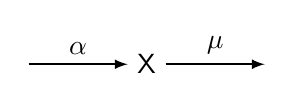
\begin{tikzpicture}
      \node (X) {X};
      \begin{scope}[semithick]
        \draw[-latex] (X) ++ (-15mm,0) -- node[midway, above] {$\alpha$} (X);
        \draw[-latex] (X) -- node[midway, above] {$\mu$} ++(15mm,0);
      \end{scope}
    \end{tikzpicture}
  \end{center}
  In this case the state space is $\mathbb{Z}_{\geq 0}$, and we can draw the
  state transitions of the dynamics with the chain below.
  \begin{center}
    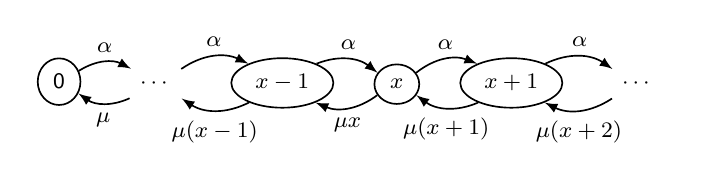
\begin{tikzpicture}
      \matrix (m) [matrix of nodes, column sep = 5mm,
        nodes = {
          draw, semithick, ellipse, minimum width = 4mm, minimum height = 4mm,
          font=\footnotesize,
        }
      ] {
        0 & |[draw=none]| $\cdots$ & $x-1$ & $x$ & $x+1$ & |[draw=none]| $\cdots$ \\
      };

      \begin{scope}[semithick, -latex, font=\footnotesize]
        \draw (m-1-1) to[bend left] node[midway, above] {$\alpha$} (m-1-2);
        \draw (m-1-2) to[bend left] node[midway, above] {$\alpha$} (m-1-3);
        \draw (m-1-3) to[bend left] node[midway, above] {$\alpha$} (m-1-4);
        \draw (m-1-4) to[bend left] node[midway, above] {$\alpha$} (m-1-5);
        \draw (m-1-5) to[bend left] node[midway, above] {$\alpha$} (m-1-6);

        \draw (m-1-6) to[bend left] node[midway, below] {$\mu (x+2)$} (m-1-5);
        \draw (m-1-5) to[bend left] node[midway, below] {$\mu (x+1)$} (m-1-4);
        \draw (m-1-4) to[bend left] node[midway, below] {$\mu x$} (m-1-3);
        \draw (m-1-3) to[bend left] node[midway, below] {$\mu (x-1)$} (m-1-2);
        \draw (m-1-2) to[bend left] node[midway, below] {$\mu$} (m-1-1);
      \end{scope}
    \end{tikzpicture}
  \end{center}
  Here simplifying the notation the CME reads
  \[
    \frac{\partial P}{\partial t}
    = \alpha P(x-1, t)  + \mu (x+1) P(x+1, t) - (\alpha + \mu x) P(x, t)
  \]
  and since we are looking for the steady state distribution $P(x)$, setting
  the above equal to zero we get the recurrence relation
  \[
    \alpha P(x-1) + \mu (x+1)  P(x+1) = (\alpha + \mu x) P(x)
  \]
  which we can solve inductively starting at $x = 0$:
  \begin{description}
    \item[$x=0:$] $\mu P(1) = \alpha P(0)$
    \item[$x=1:$] \begin{align*}
        \alpha P(0) + 2\mu P(2) &= (\alpha + \mu) P(1) \\
          &= \alpha P(1) + \alpha P(0) \\
        \Rightarrow \quad 2\mu P(2) = \alpha P(1)
    \end{align*}
    \item[$x=2:$] \begin{align*}
        \alpha P(1) + 3\mu P(3) &= (\alpha + 2\mu) P(2) \\
          &= \alpha P(2) + \alpha P(1) \\
        \Rightarrow \quad 3\mu P(3) = \alpha P(2)
    \end{align*}
  \end{description}
  the pattern continues with
  \begin{gather*}
    x\mu P(x) = \alpha P(x-1) \\
    \Rightarrow \quad
    P(x) = \frac{\alpha}{\mu x} P(x-1) = 
    \left( \frac{\alpha}{\mu} \right)^x \frac{1}{x!} P(0),
  \end{gather*}
  and then because $P(x)$ is a probability distribution it must be that
  \[
    \sum_{x \in \mathbb{Z}_{\geq 0}} P(x) 
      = \sum_{x = 0}^\infty \left( \frac{\alpha}{\mu} \right)^x \frac{1}{x!}
      P(0) = 1
  \]
  and we can solve for $P(0)$ and find $P(0) = e^{-\alpha / \mu}$. If we take
  the expectation of the state in steady state we recover the deterministic
  result
  \begin{align*}
    \E{x} &= \sum_{x \in \mathbb{Z}_{\geq 0}} x P(x)
      = \sum_{x = 0}^\infty x \left(
        \frac{\alpha}{\mu}
      \right)^x \frac{1}{x!} P(0) \\
    &= \frac{\alpha}{\mu} \sum_{x = 0}^\infty x \left(
        \frac{\alpha}{\mu}
      \right)^{x-1} \frac{P(0)}{(x-1)!} 
    = \frac{\alpha}{\mu} e^{\alpha/\mu} P(0) = \frac{\alpha}{\mu}.
  \end{align*}
\end{example}

As done in the example with the CME it is theoretically possible to compute
the distribution of moments for the states, for instance the average molecule
numbers have dynamics
\[
  \frac{d}{dt} \langle n_i(t) \rangle = \sum_{j=1}^M \nu_{ij} \langle
  a_j(n(t)) \rangle.
\]
If all propensity functions $a_j$ are linear in the state variable $n$ (this
happens when there are only unimolecular reactions) the expectation commutes
and we have that $\langle a_j(n(t)) \rangle = a_j (\langle n(t) \rangle )$.
In the presence of bimolecular (or more complex) reactions there is no
analytical solution.

\subsection{Stochastic Simulation}

Since analytically solving the CME is practically impossible the idea of a
stochastic simulation is to determine a set of representative trajectories
instead of solving for the probability density. We will discuss Gillespie's
algorithm.

The starting point is a state $n$ at time $t$. To simulate the system to the
next step we define $\tau$ as the time at which the next time occurs, and $j$
the index of that reaction. We write
\[
  P(\tau, j \given n, t) d\tau
\]
to denote the joint PDF in $\tau$ (continuous) and $j$ (discrete) that the
next reaction will occur in the time interval $[t + \tau, t + \tau + d\tau)$,
and that it will be a reaction of type $R_j$.

\todo{Gillespie}

\end{document}
% vim:ts=2 sw=2 et tw=78 spell spelllang=en:
